\documentclass[twocolumn]{article}
\setlength\columnseprule{1pt}
\usepackage{array}
\usepackage{graphicx}
\graphicspath{ {./images/} }
\title{White Car}


\begin{document}

\maketitle

\begin{center}
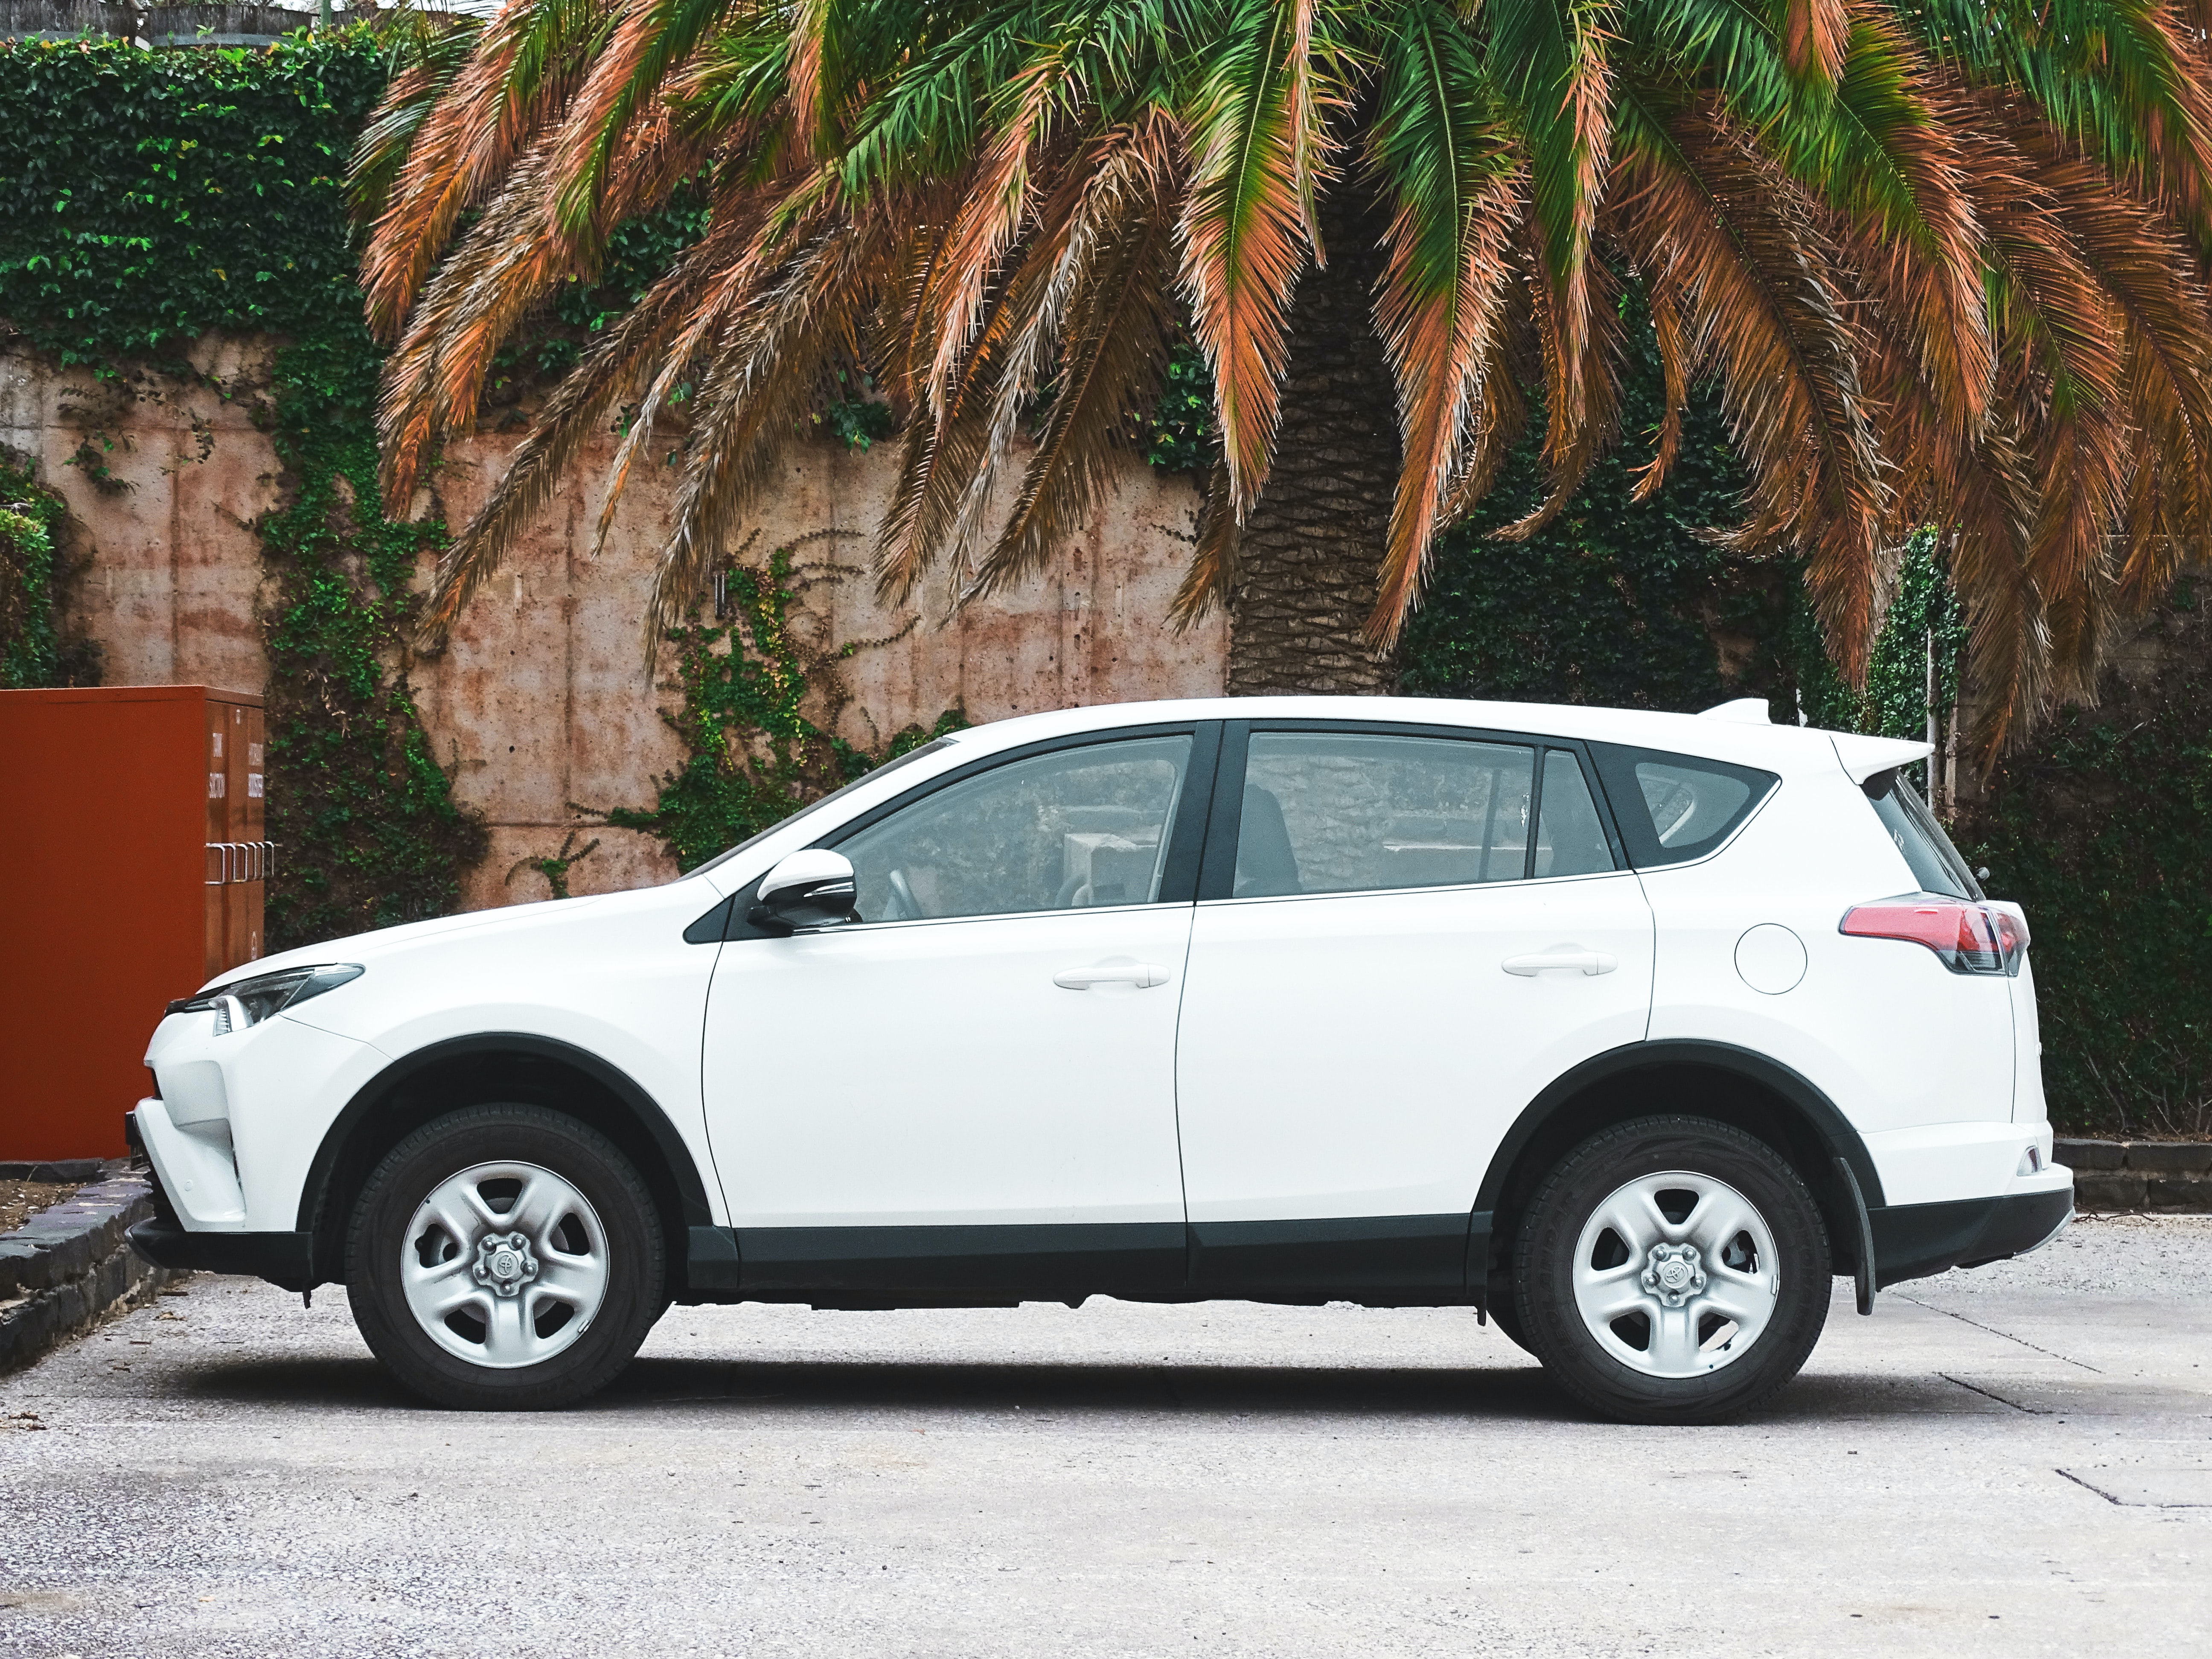
\includegraphics[width=0.7\columnwidth]{Image1}

%


\begin{tabular}{| m{3cm} | m{3cm} |}
\hline

Title  &  Value   \\

\hline
Camera Make  & SONY   \\
\hline
Camera Model  & DSC-HX400V   \\
\hline
Exposure time  & 1/640  \\
\hline
aperture & 4.0 \\
\hline


\end{tabular}


\end{center}

\pagebreak

\begin{center}
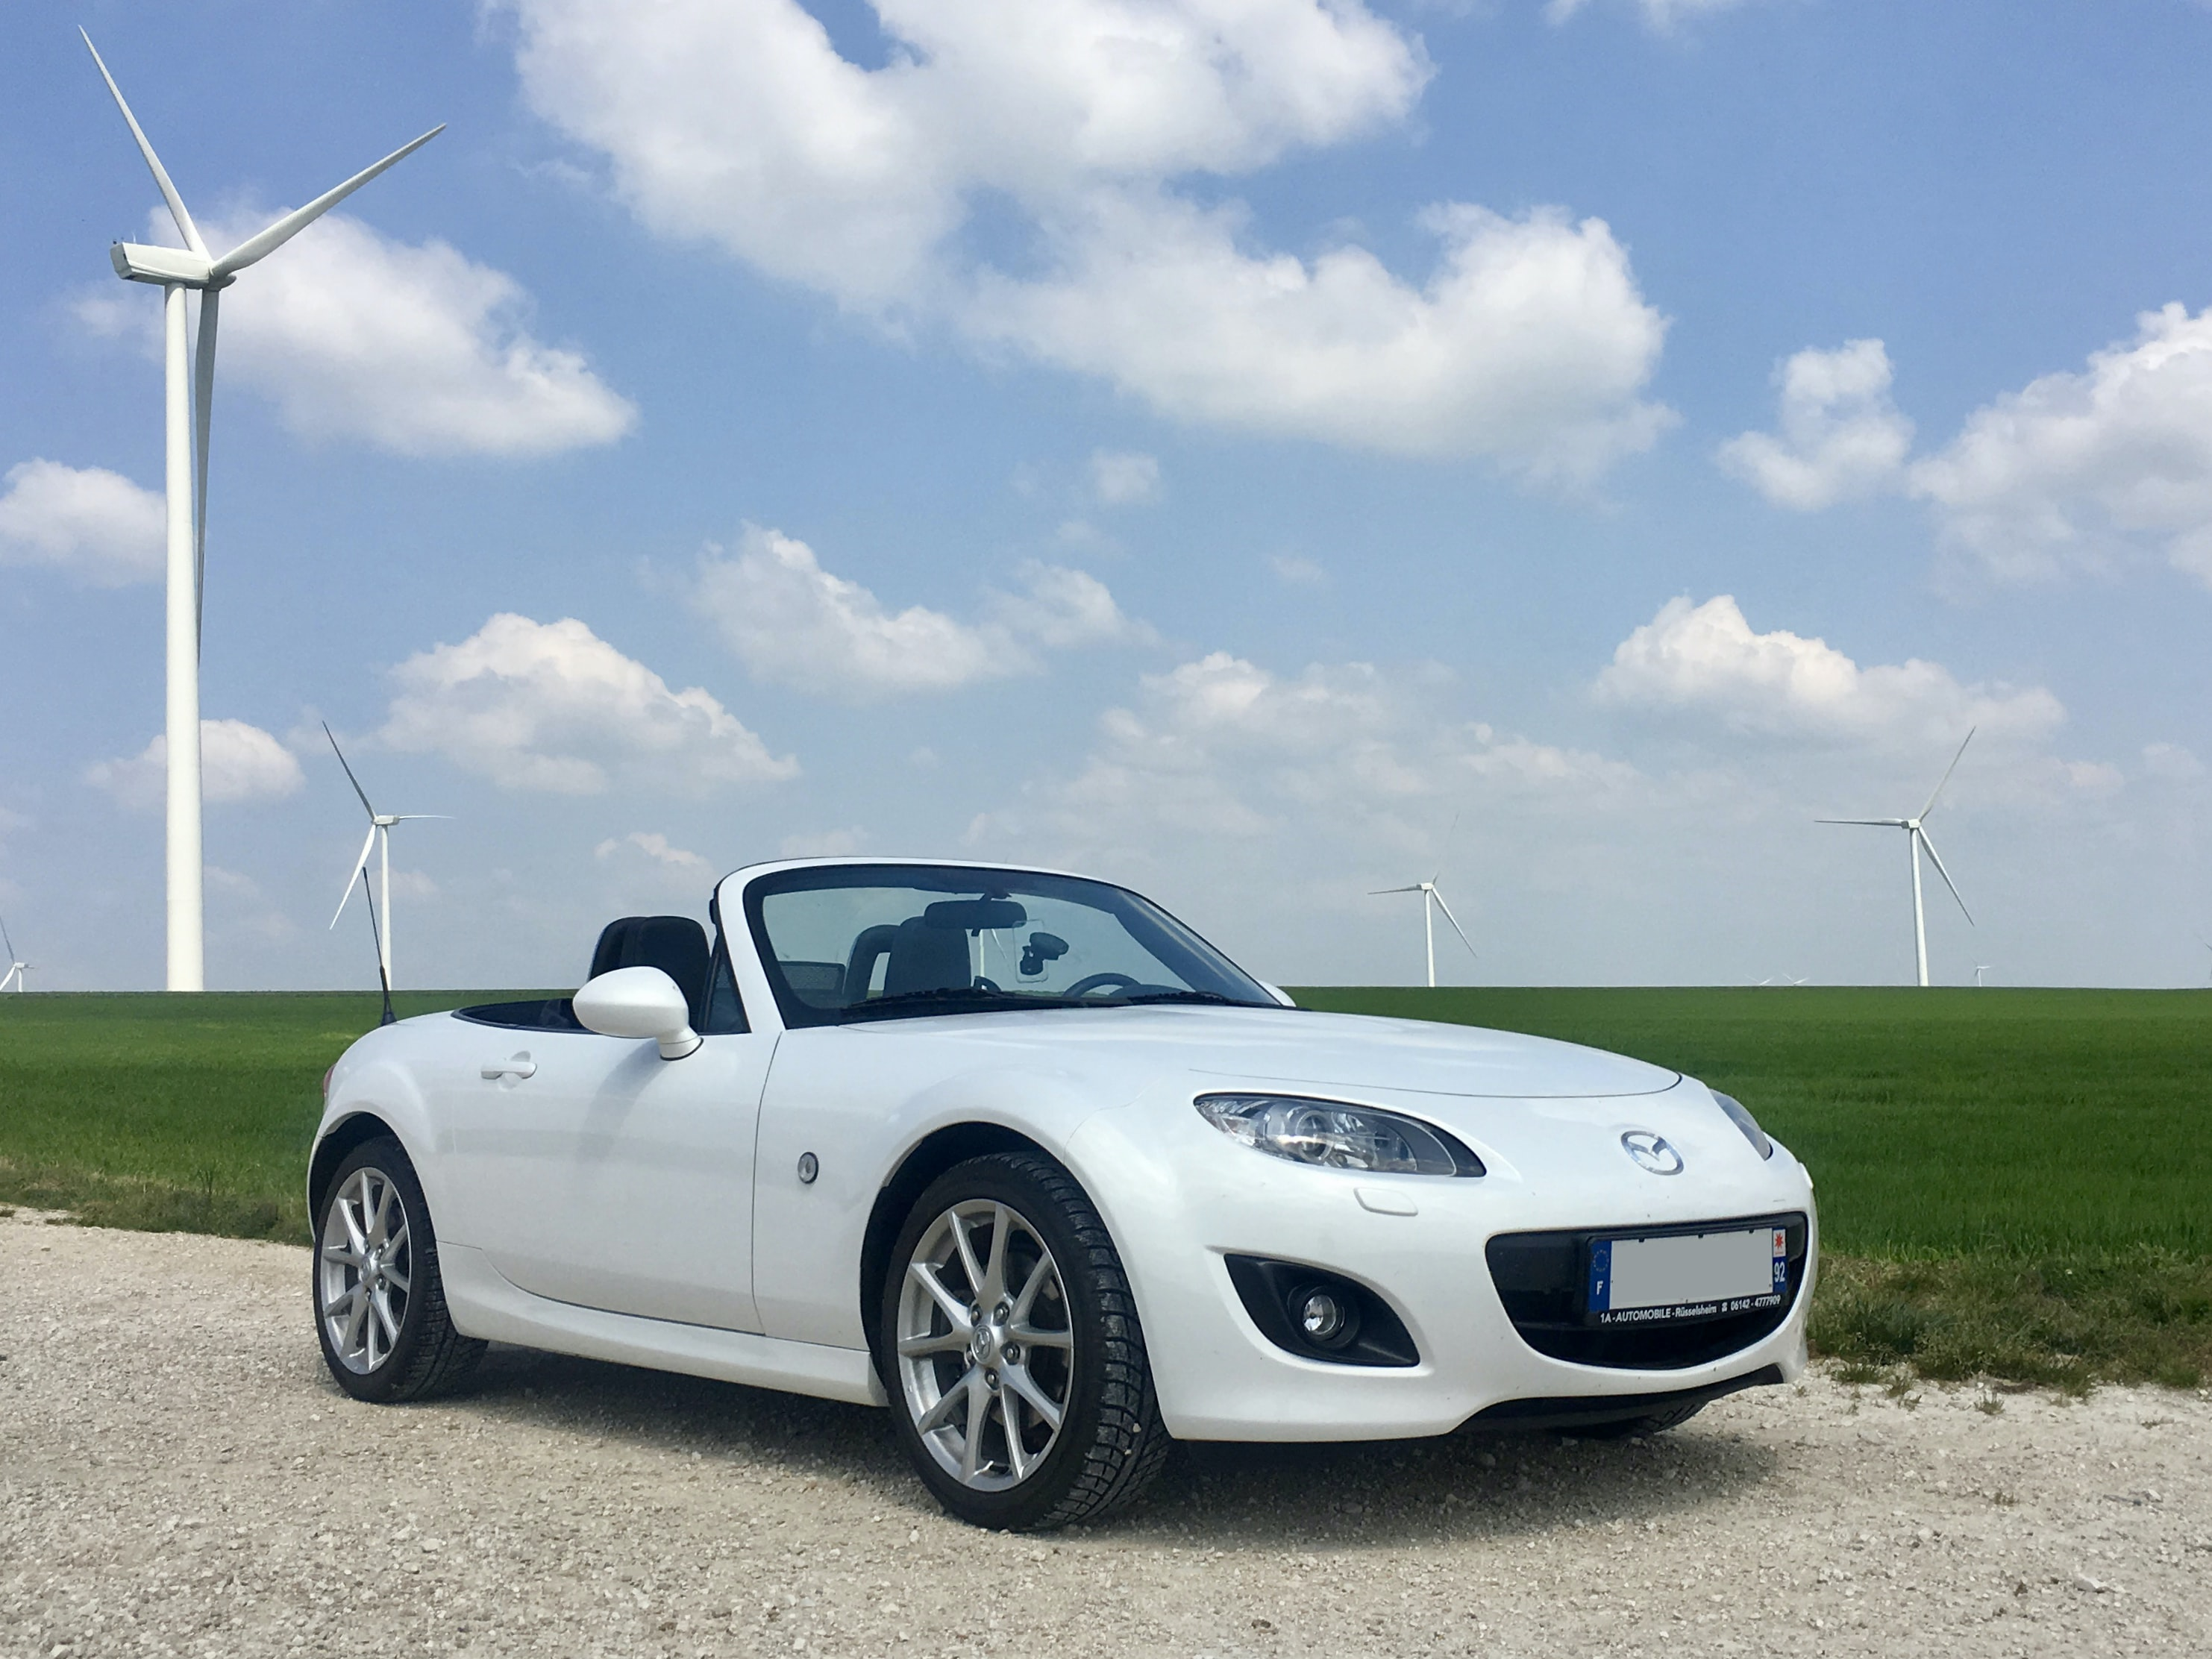
\includegraphics[width=0.7\columnwidth]{Image2}
\newline
\newline
\newline
\newline
\newline

\begin{tabular}{| m{3cm} | m{3cm} |}
\hline

Title  &  Value   \\

\hline
Camera Make  & Apple   \\
\hline
Camera Model  & iPhone 6s   \\
\hline
Exposure time  & 1/3077  \\
\hline
aperture & 2.2 \\
\hline

\end{tabular}


\end{center}

\newpage

\begin{center}
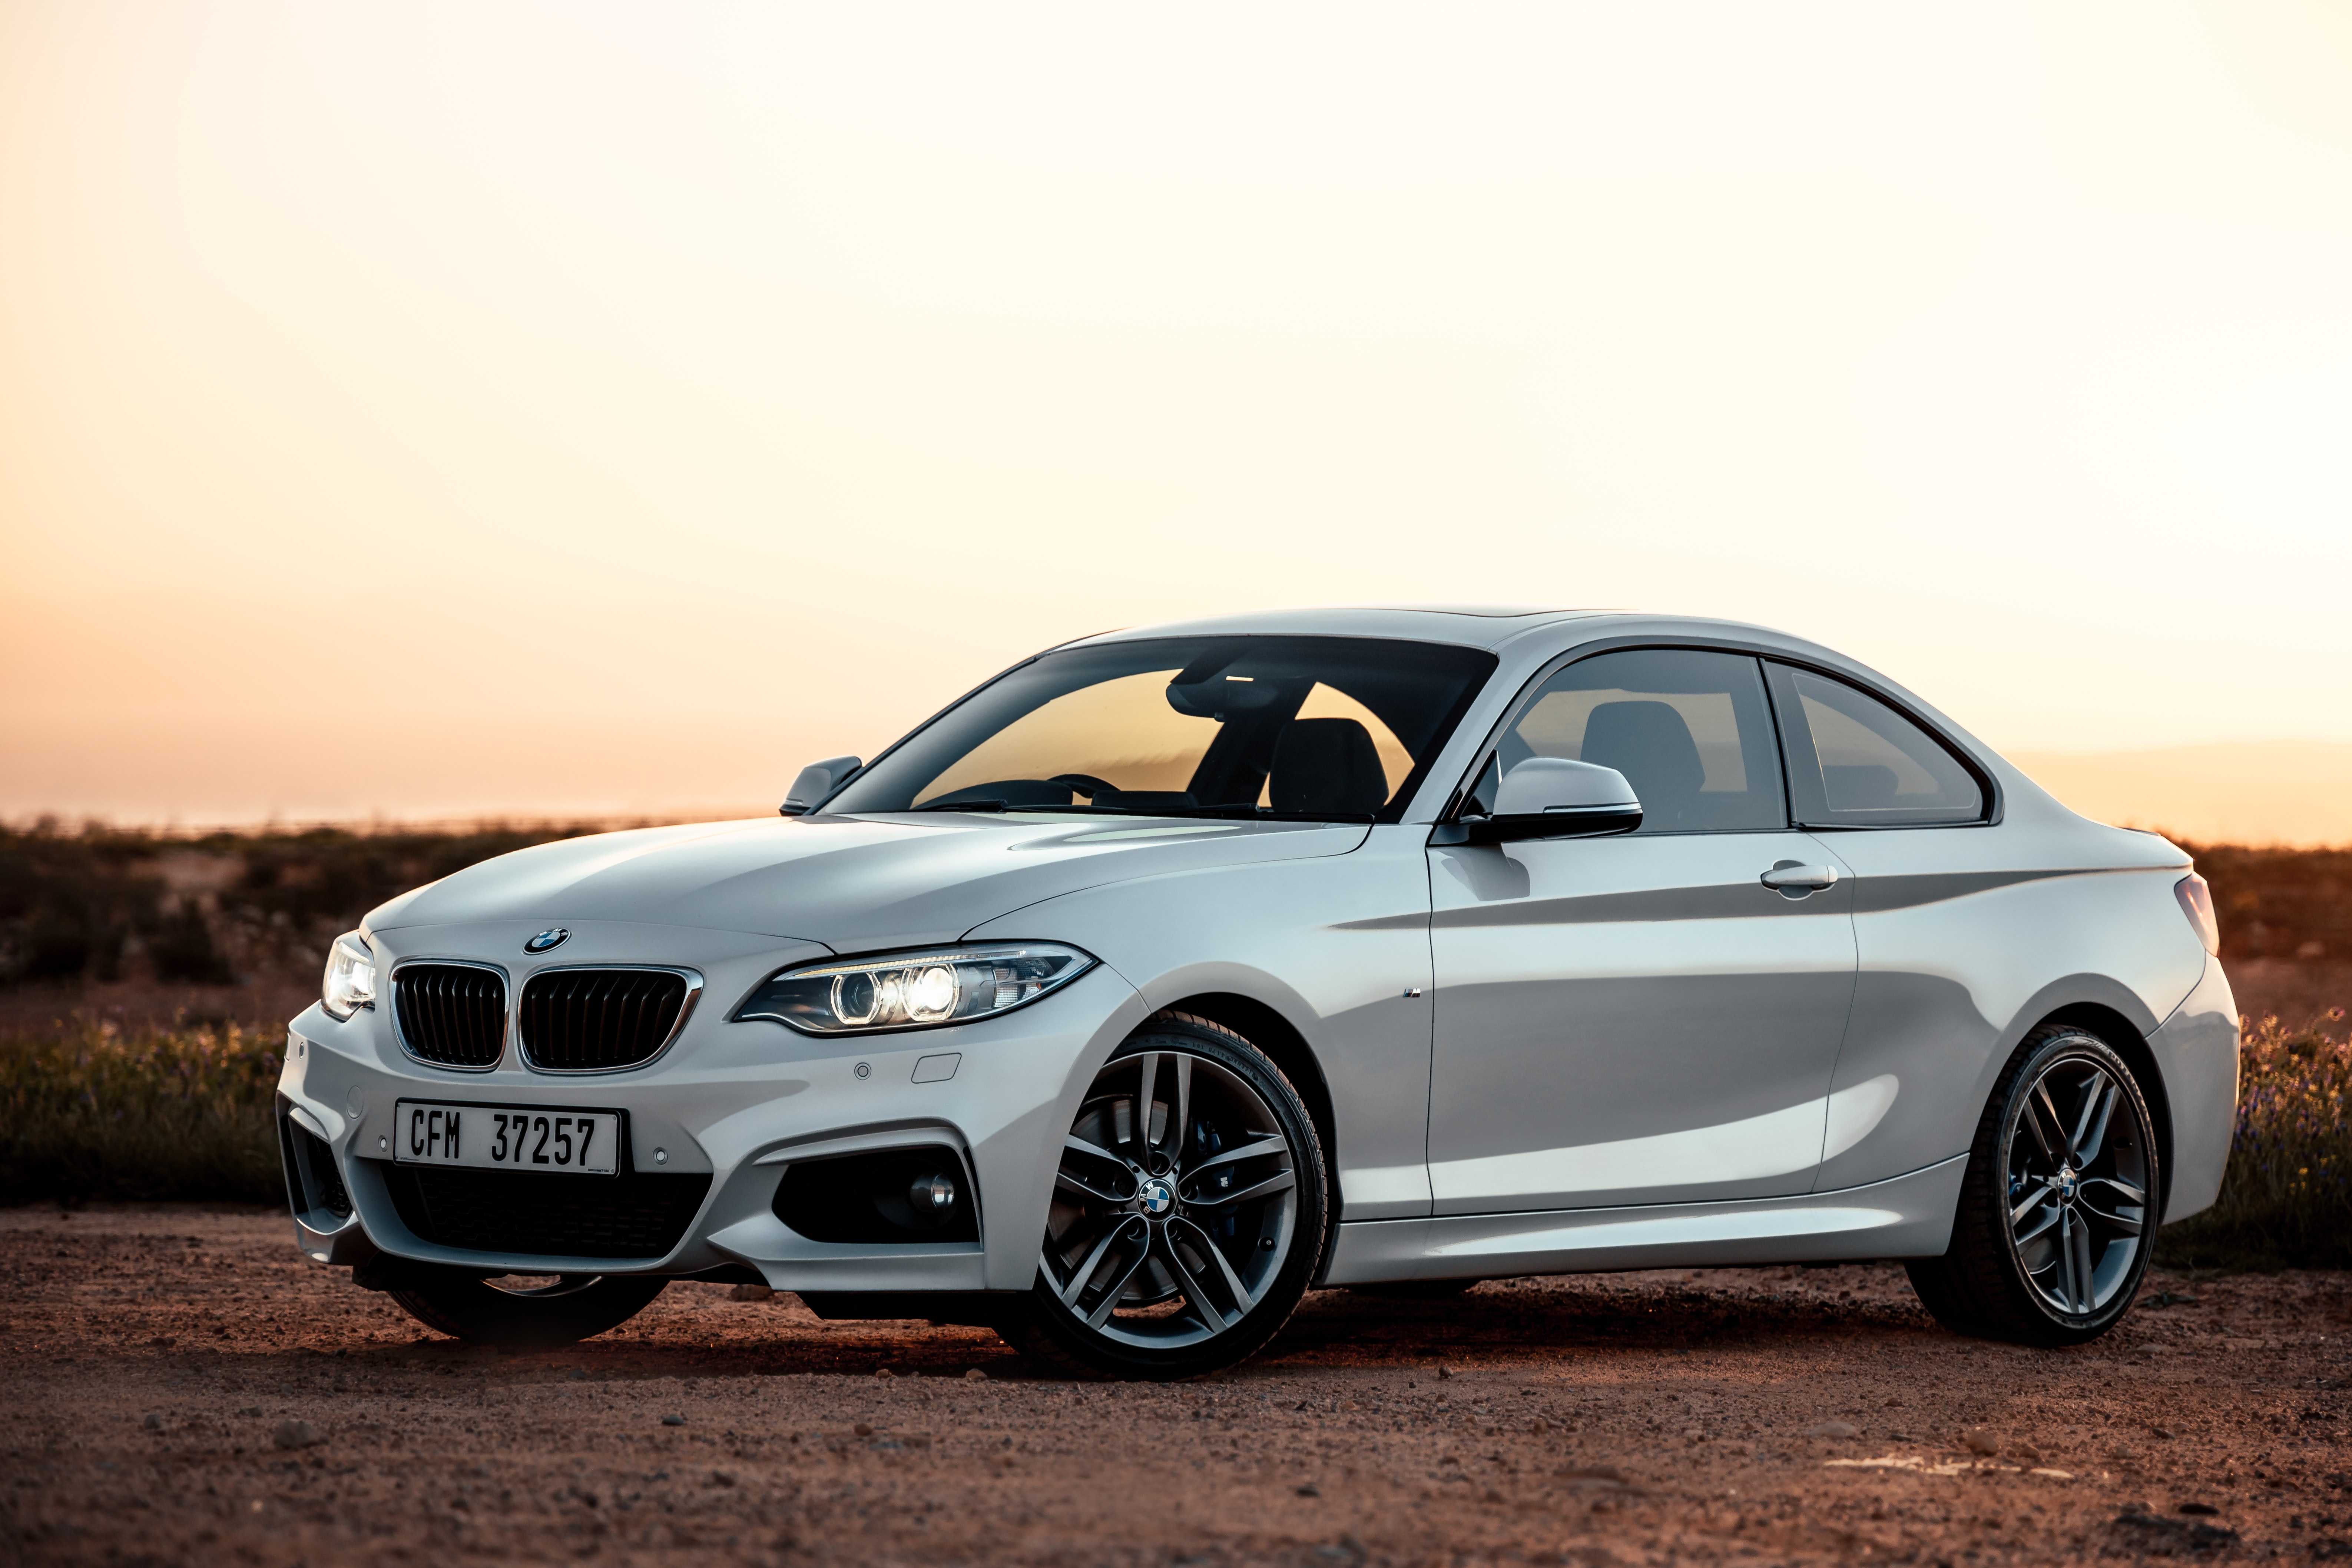
\includegraphics[width=0.7\columnwidth]{Image3}
\newline
\newline
\newline
\newline
\newline
\begin{tabular}{| m{3cm} | m{3cm} |}
\hline

Title  &  Value   \\

Title  &  Value   \\

\hline
Camera Make  & Canon   \\
\hline
Camera Model  & Canon EOS R   \\
\hline
Exposure time  & 1/80  \\
\hline
aperture & 4.0 \\
\hline


\end{tabular}


\end{center}

\pagebreak

\begin{center}
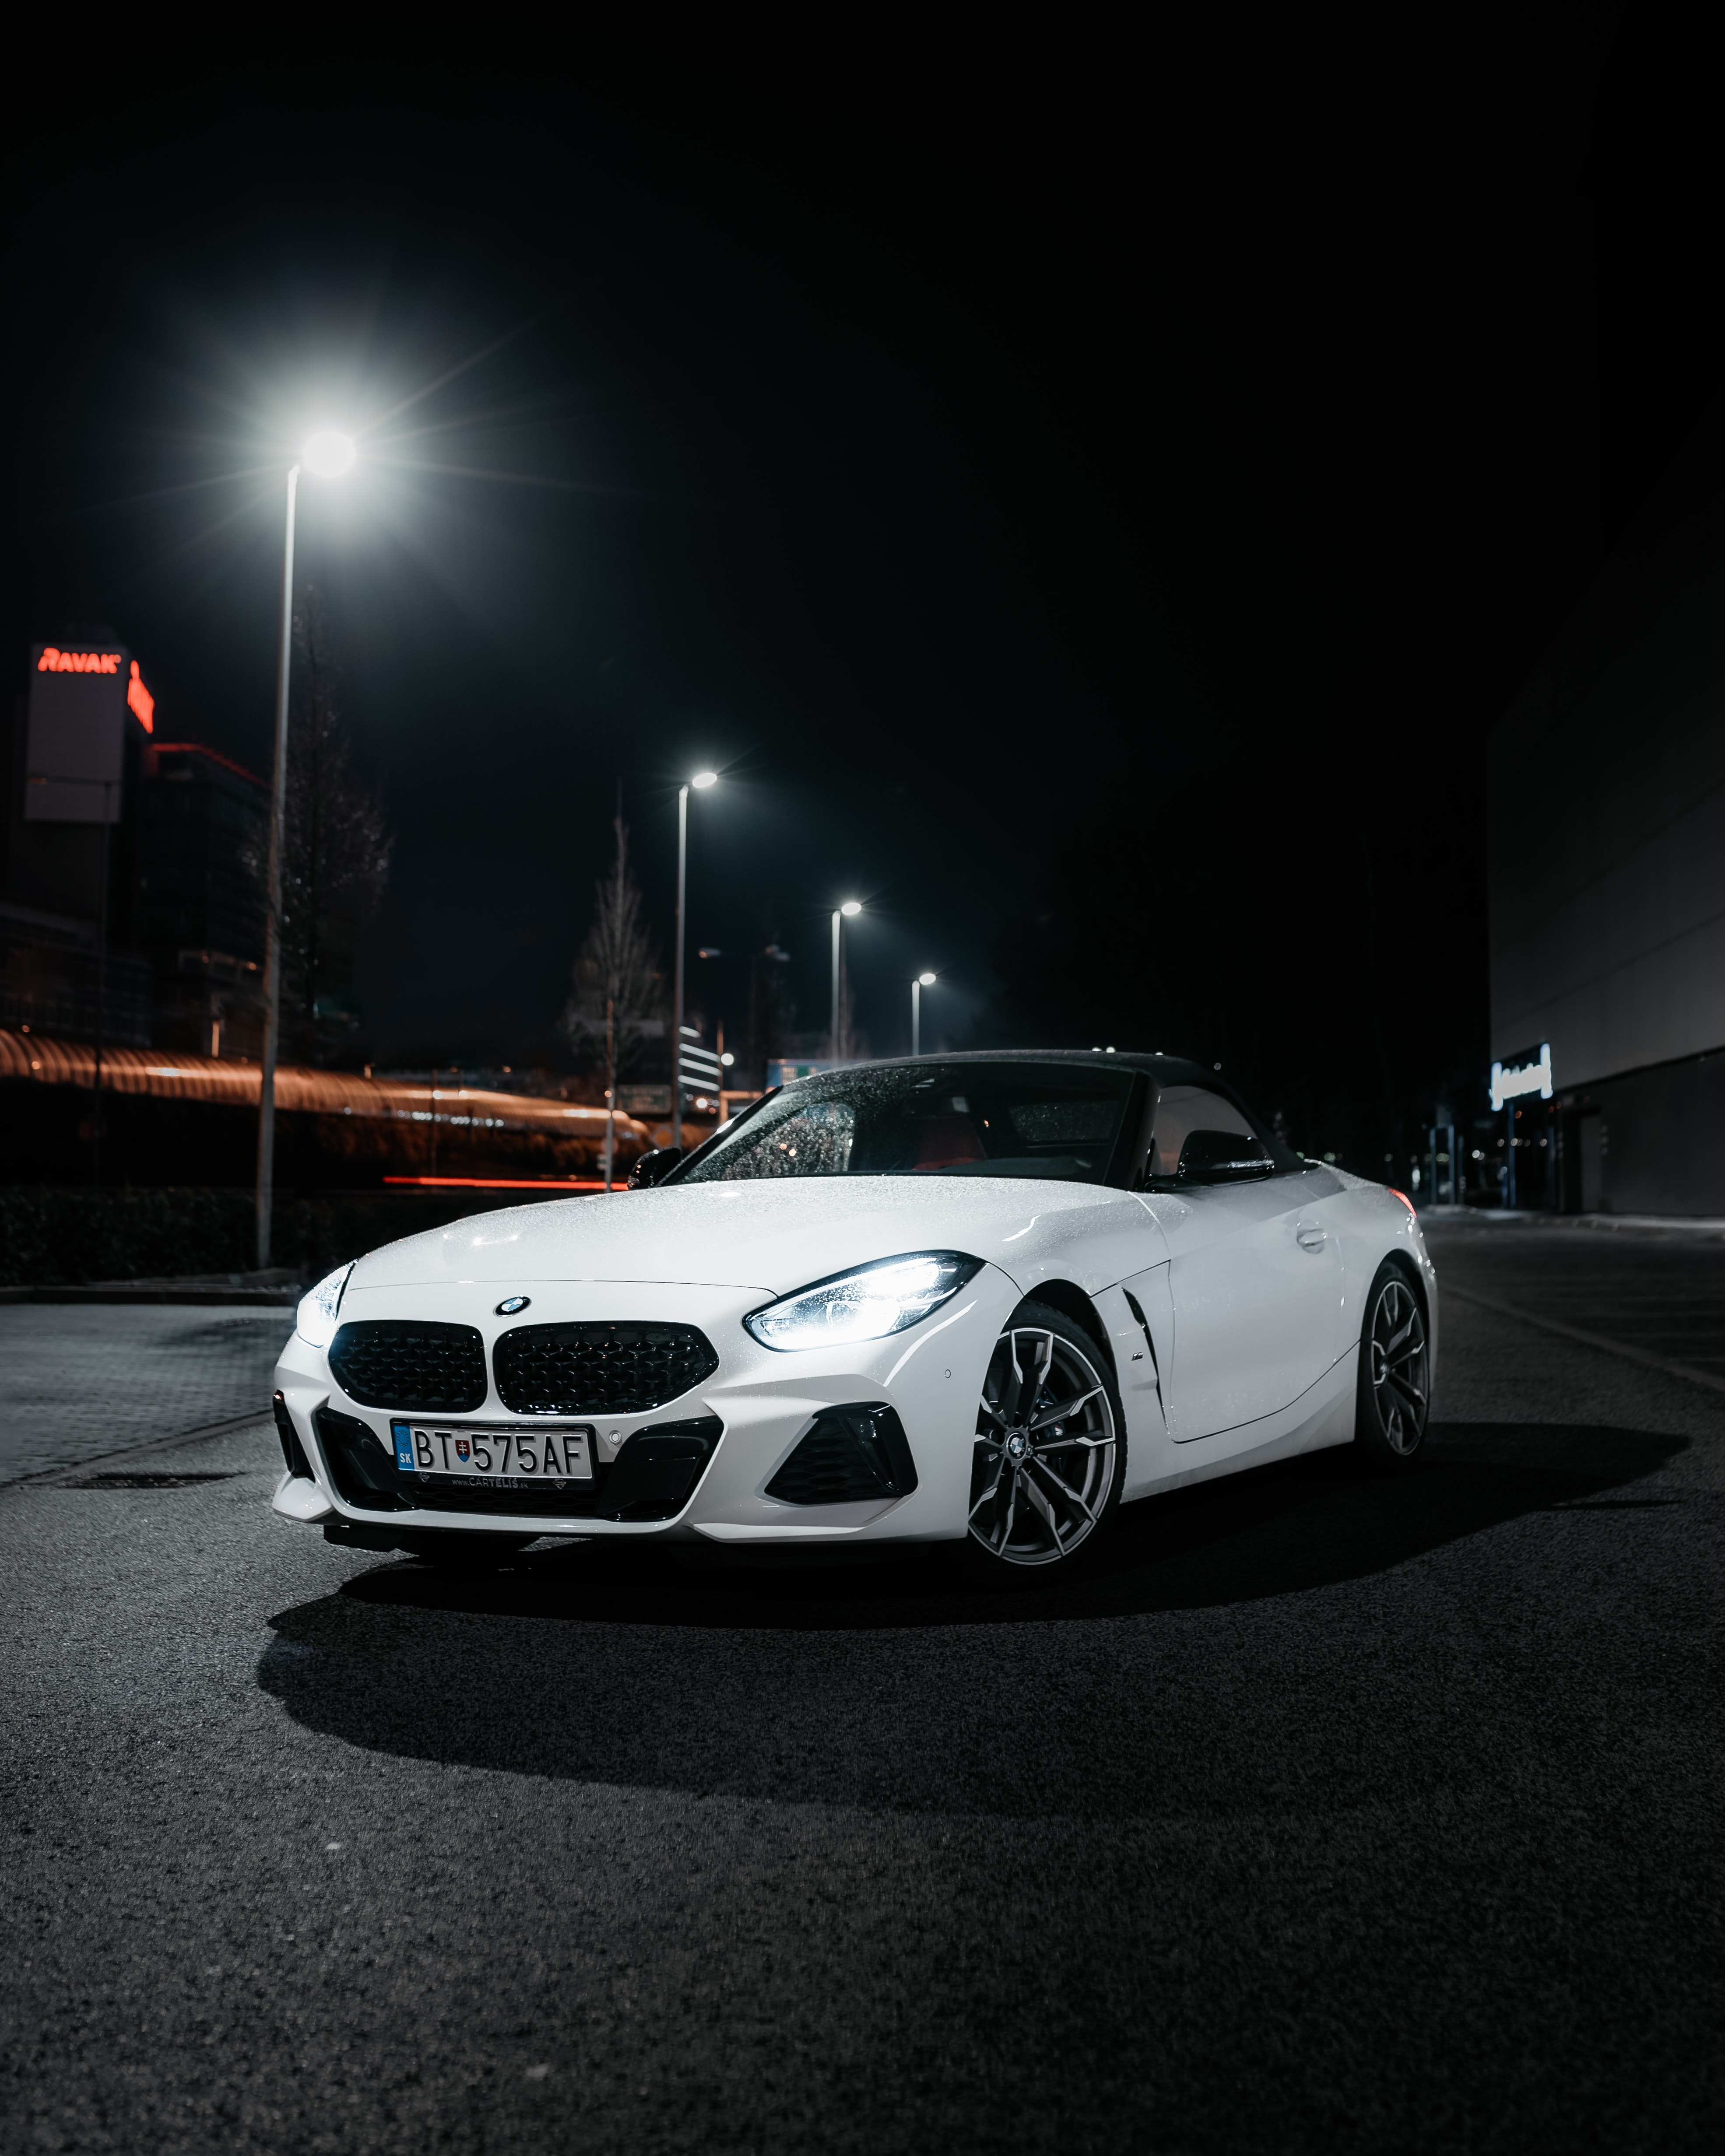
\includegraphics[width=0.7\columnwidth]{Image4}
\newline
\newline
\newline
\newline
\newline

\begin{tabular}{| m{3cm} | m{3cm} |}
\hline

Title  &  Value   \\

\hline
Camera Make  & Canon   \\
\hline
Camera Model  & Canon EOS R   \\
\hline
Exposure time  & 1.6  \\
\hline
aperture & 2.5 \\
\hline

\end{tabular}


\end{center}

\newpage

\begin{center}
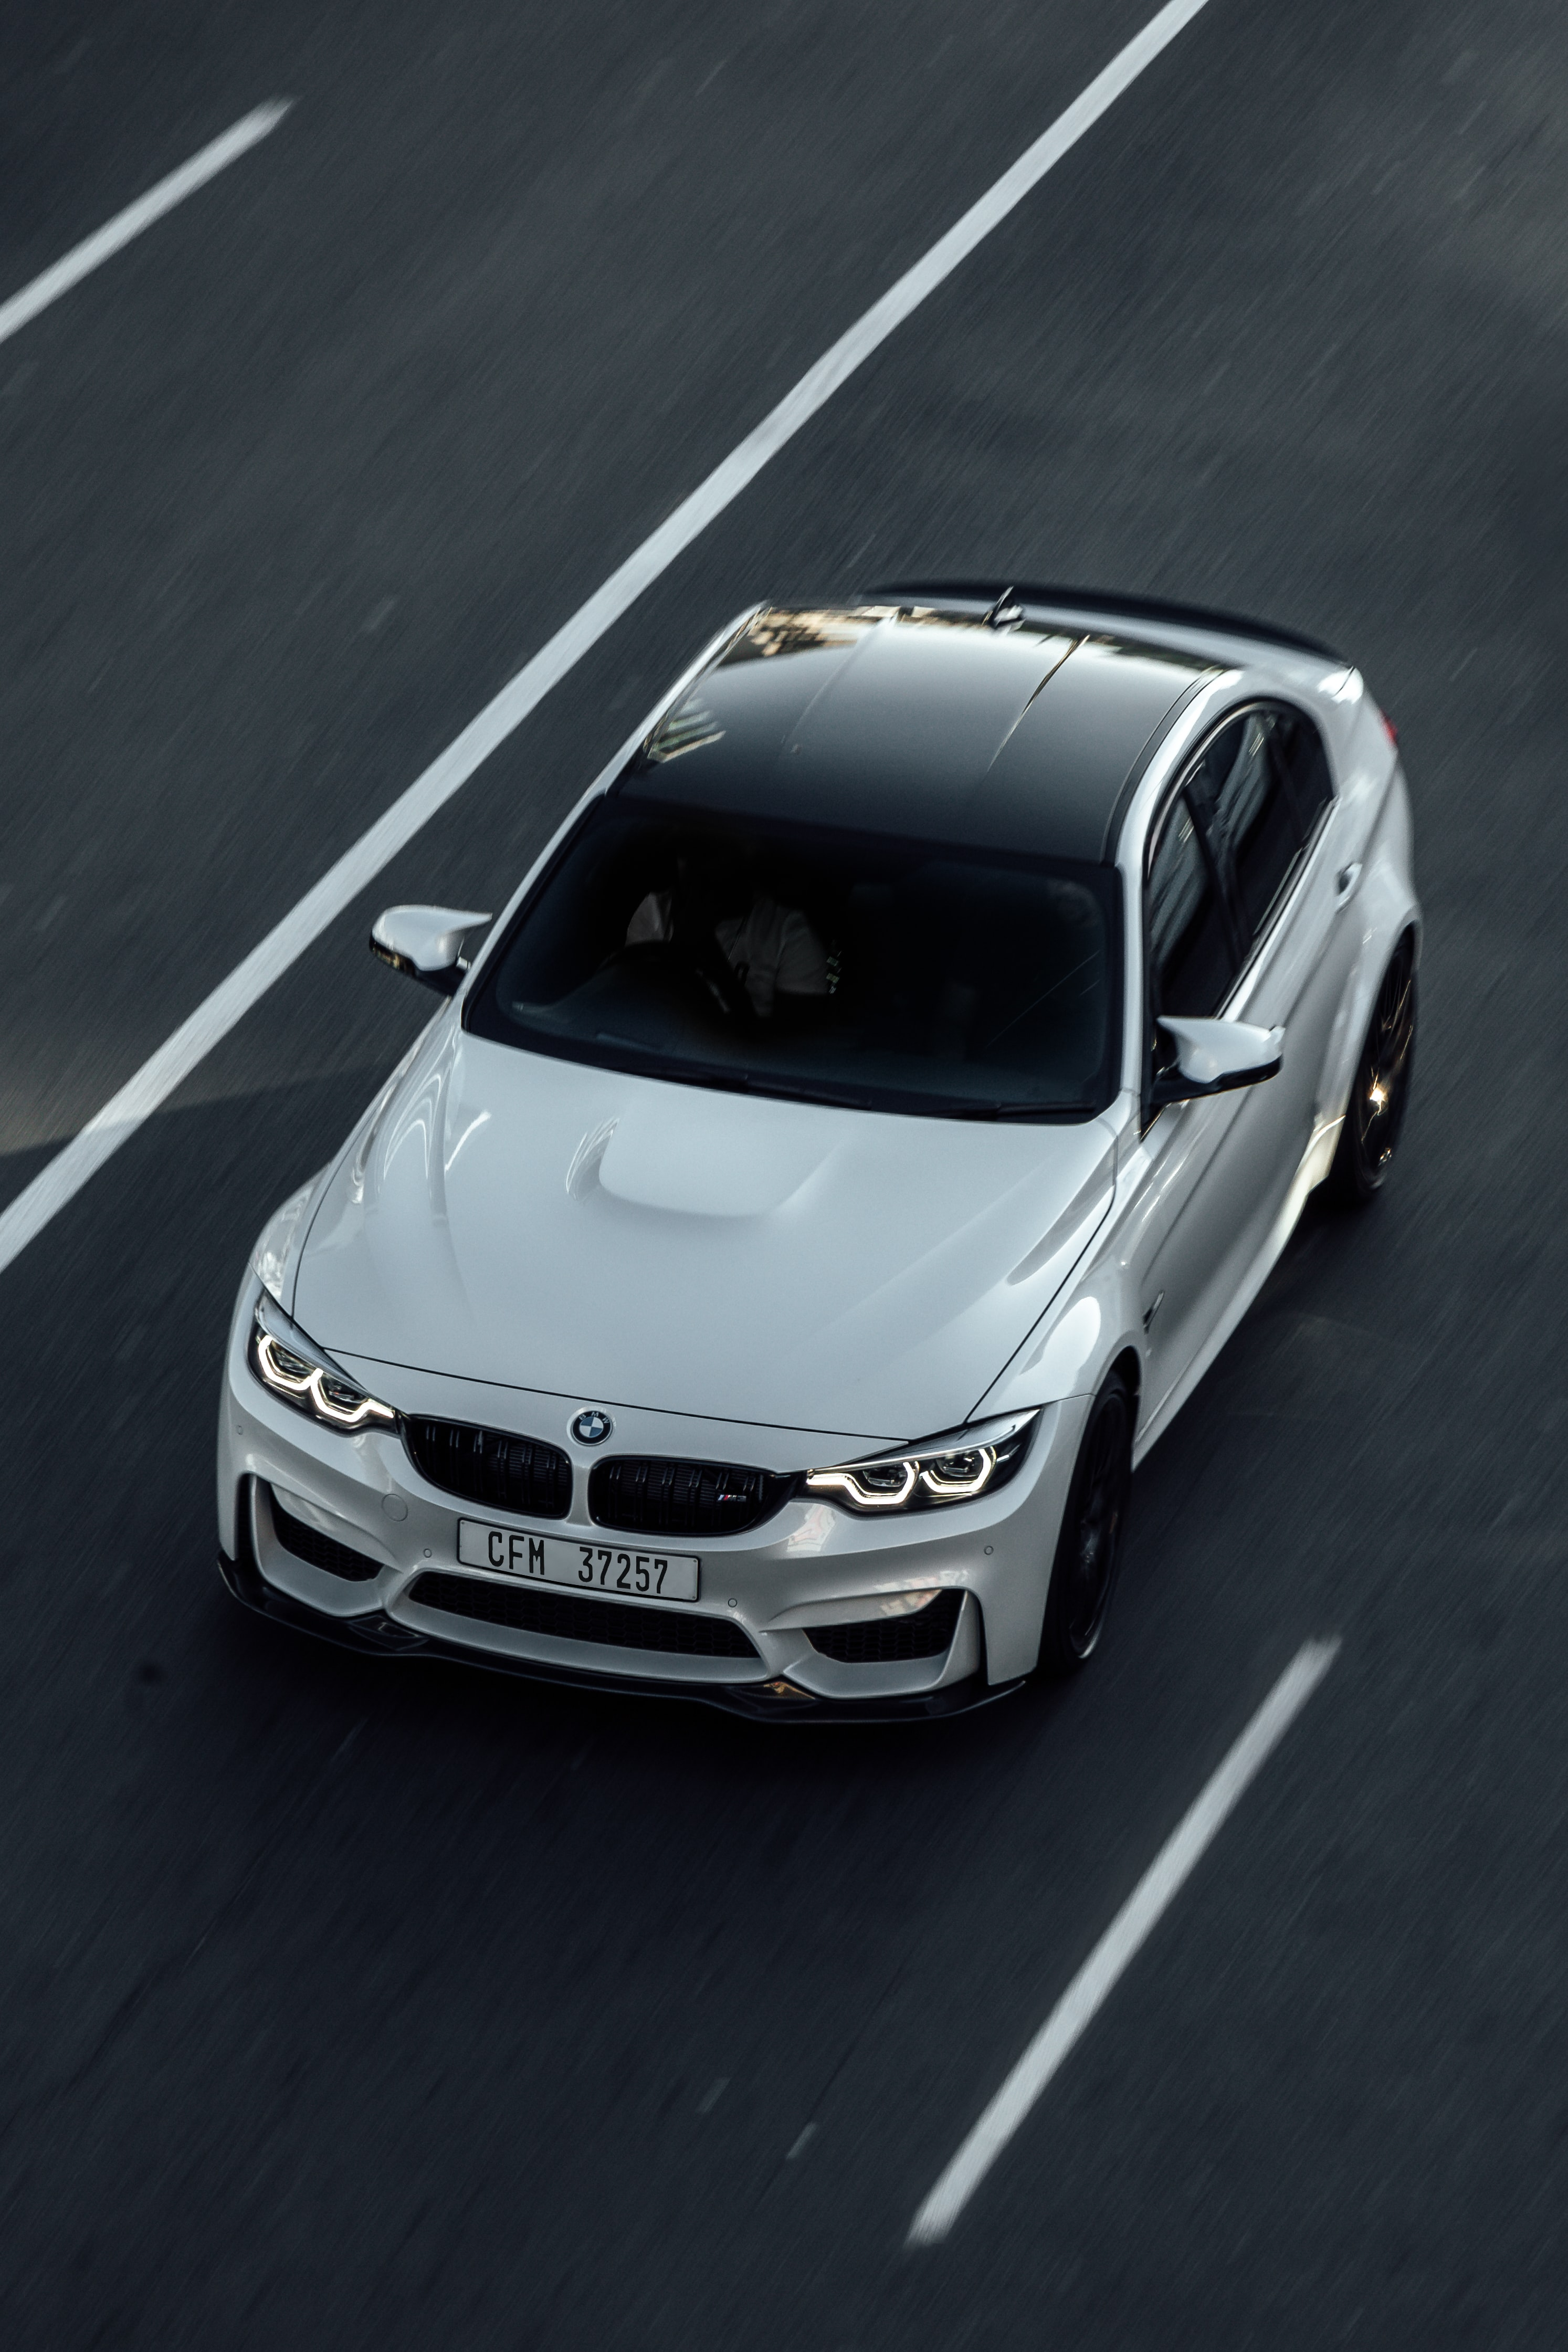
\includegraphics[width=0.7\columnwidth]{Image5}
\newline
\newline
\newline
\newline
\newline
\begin{tabular}{| m{3cm} | m{3cm} |}
\hline

Title  &  Value   \\

\hline
Camera Make  & Canon   \\
\hline
Camera Model  & Canon EOS R   \\
\hline
Exposure time  & 1/50  \\
\hline
aperture & 13.0 \\
\hline


\end{tabular}


\end{center}

\pagebreak

\begin{center}
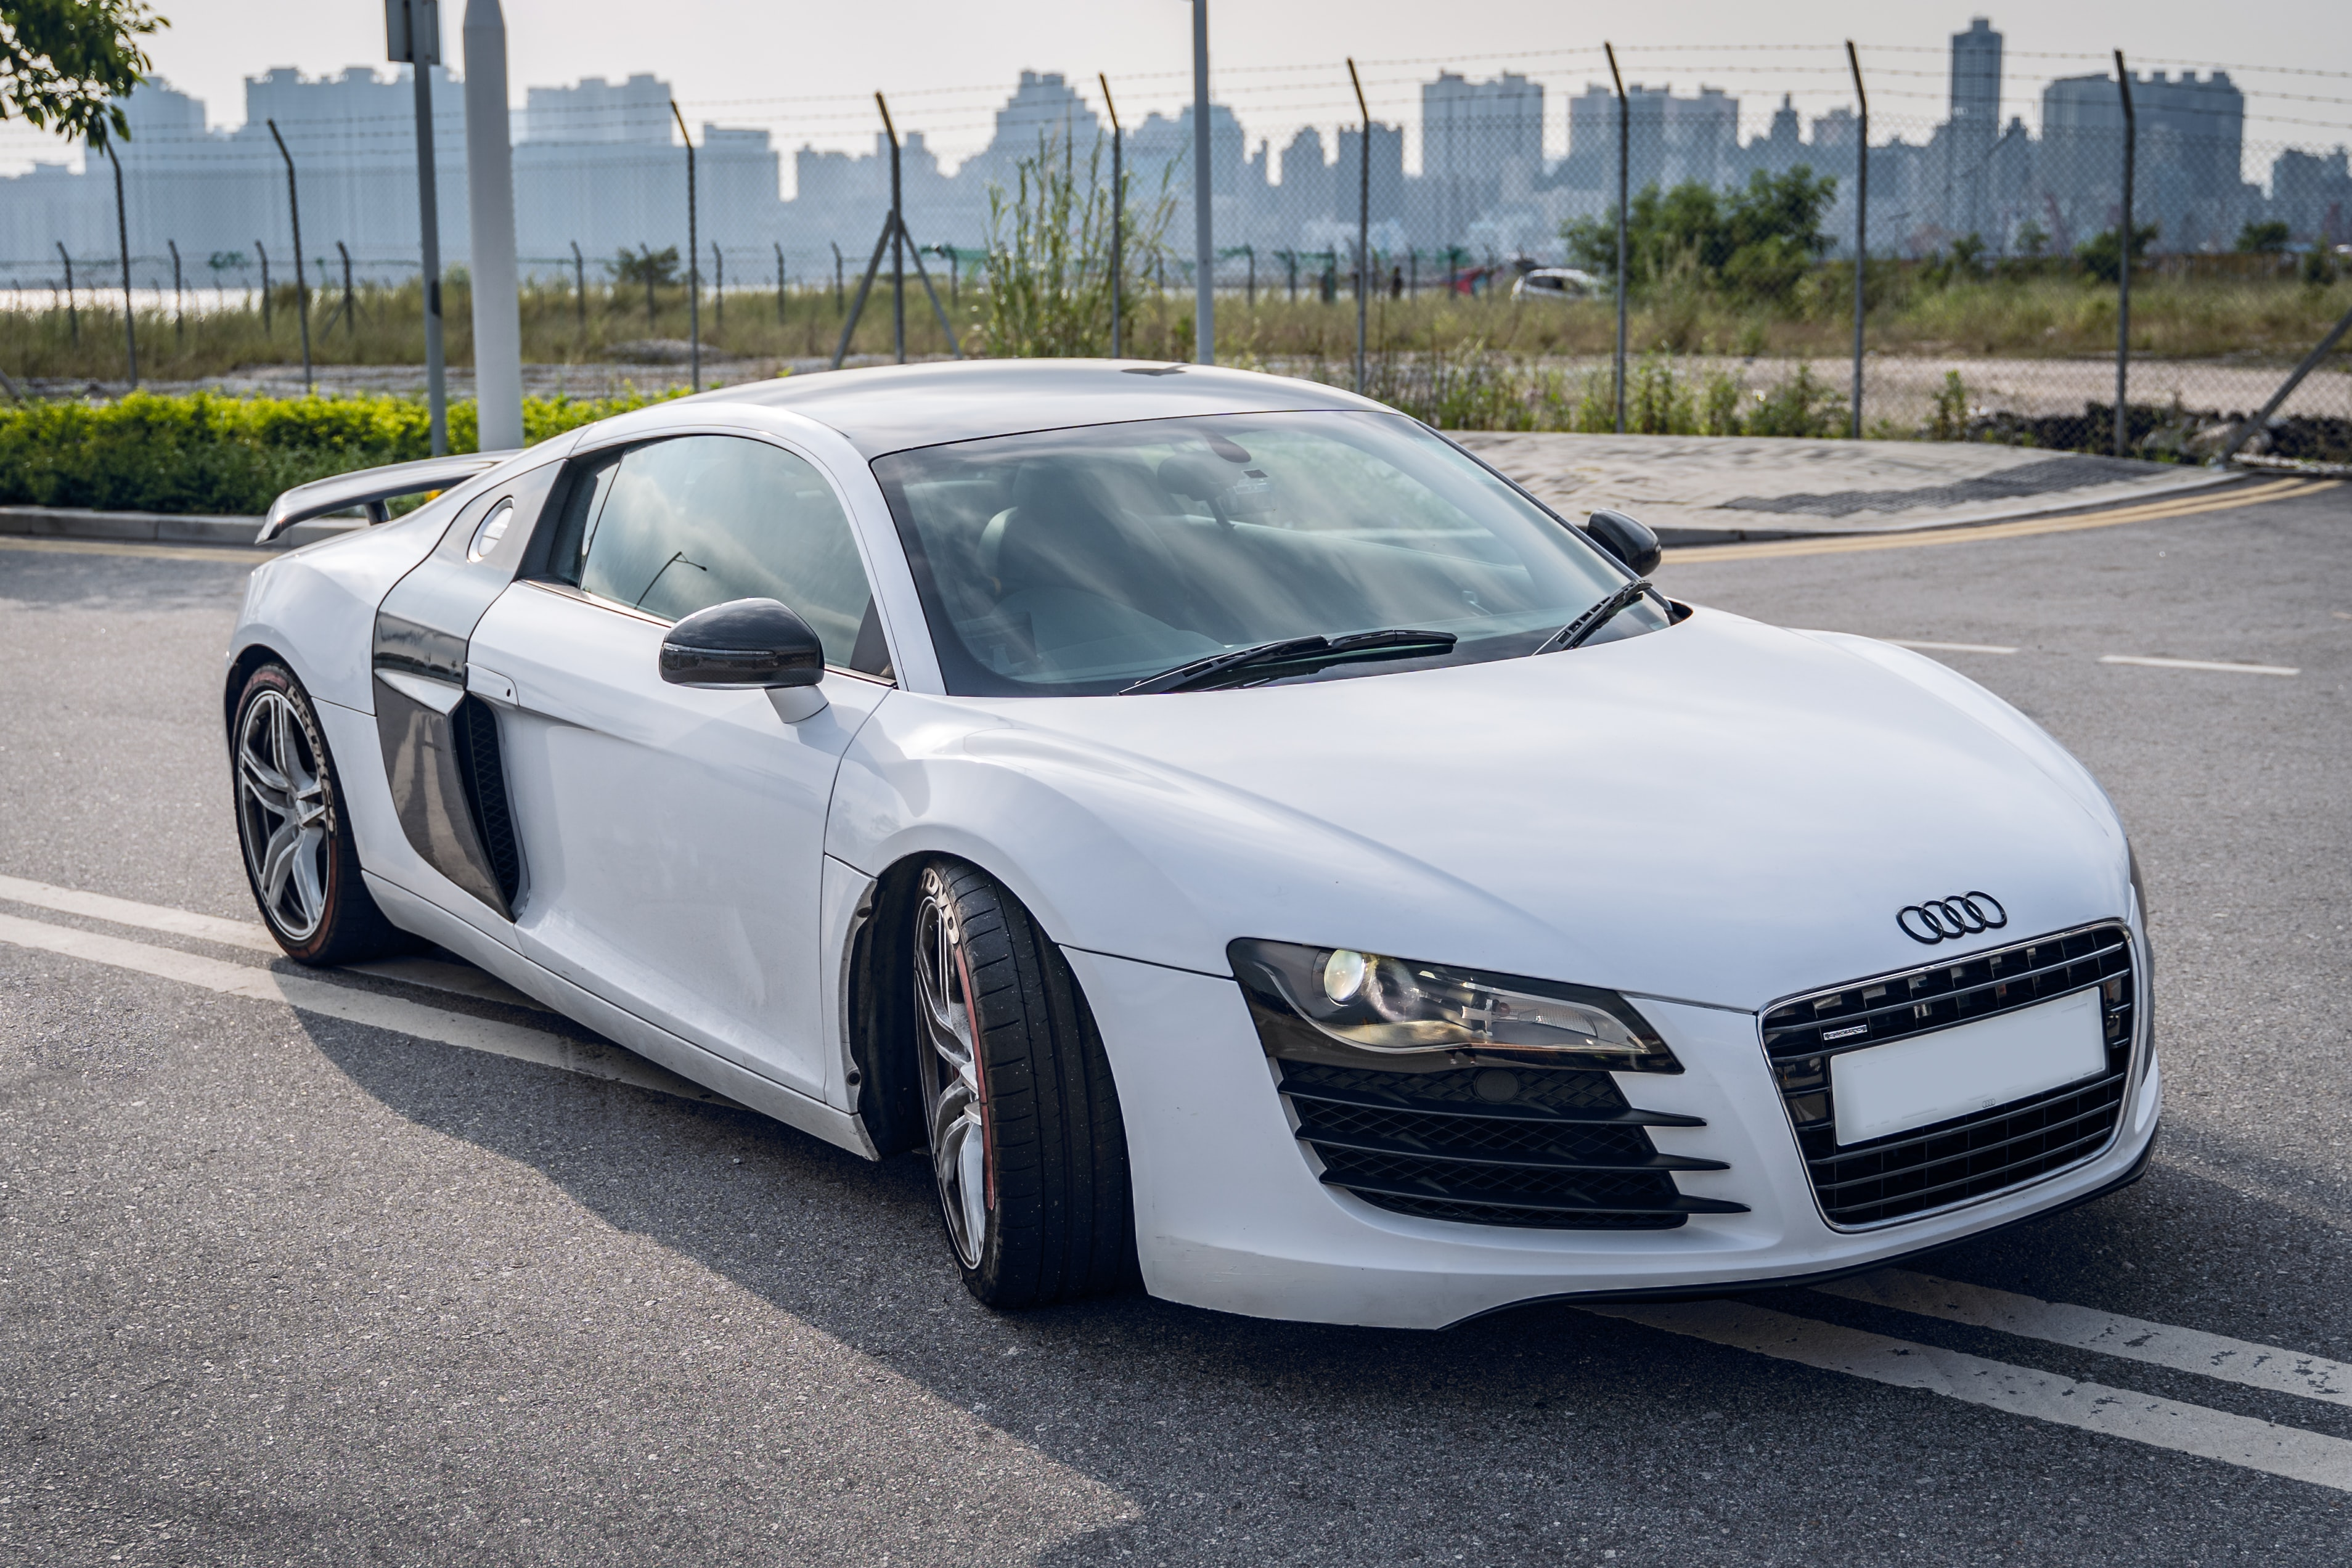
\includegraphics[width=0.7\columnwidth]{Image6}
\newline
\newline
\newline
\newline
\newline

\begin{tabular}{| m{3cm} | m{3cm} |}
\hline

Title  &  Value   \\

\hline
Camera Make  & SONY   \\
\hline
Camera Model  & ILCE-7M3   \\
\hline
Exposure time  & 1/1600  \\
\hline
aperture & 2.8 \\
\hline

\end{tabular}


\end{center}

\newpage

\begin{center}
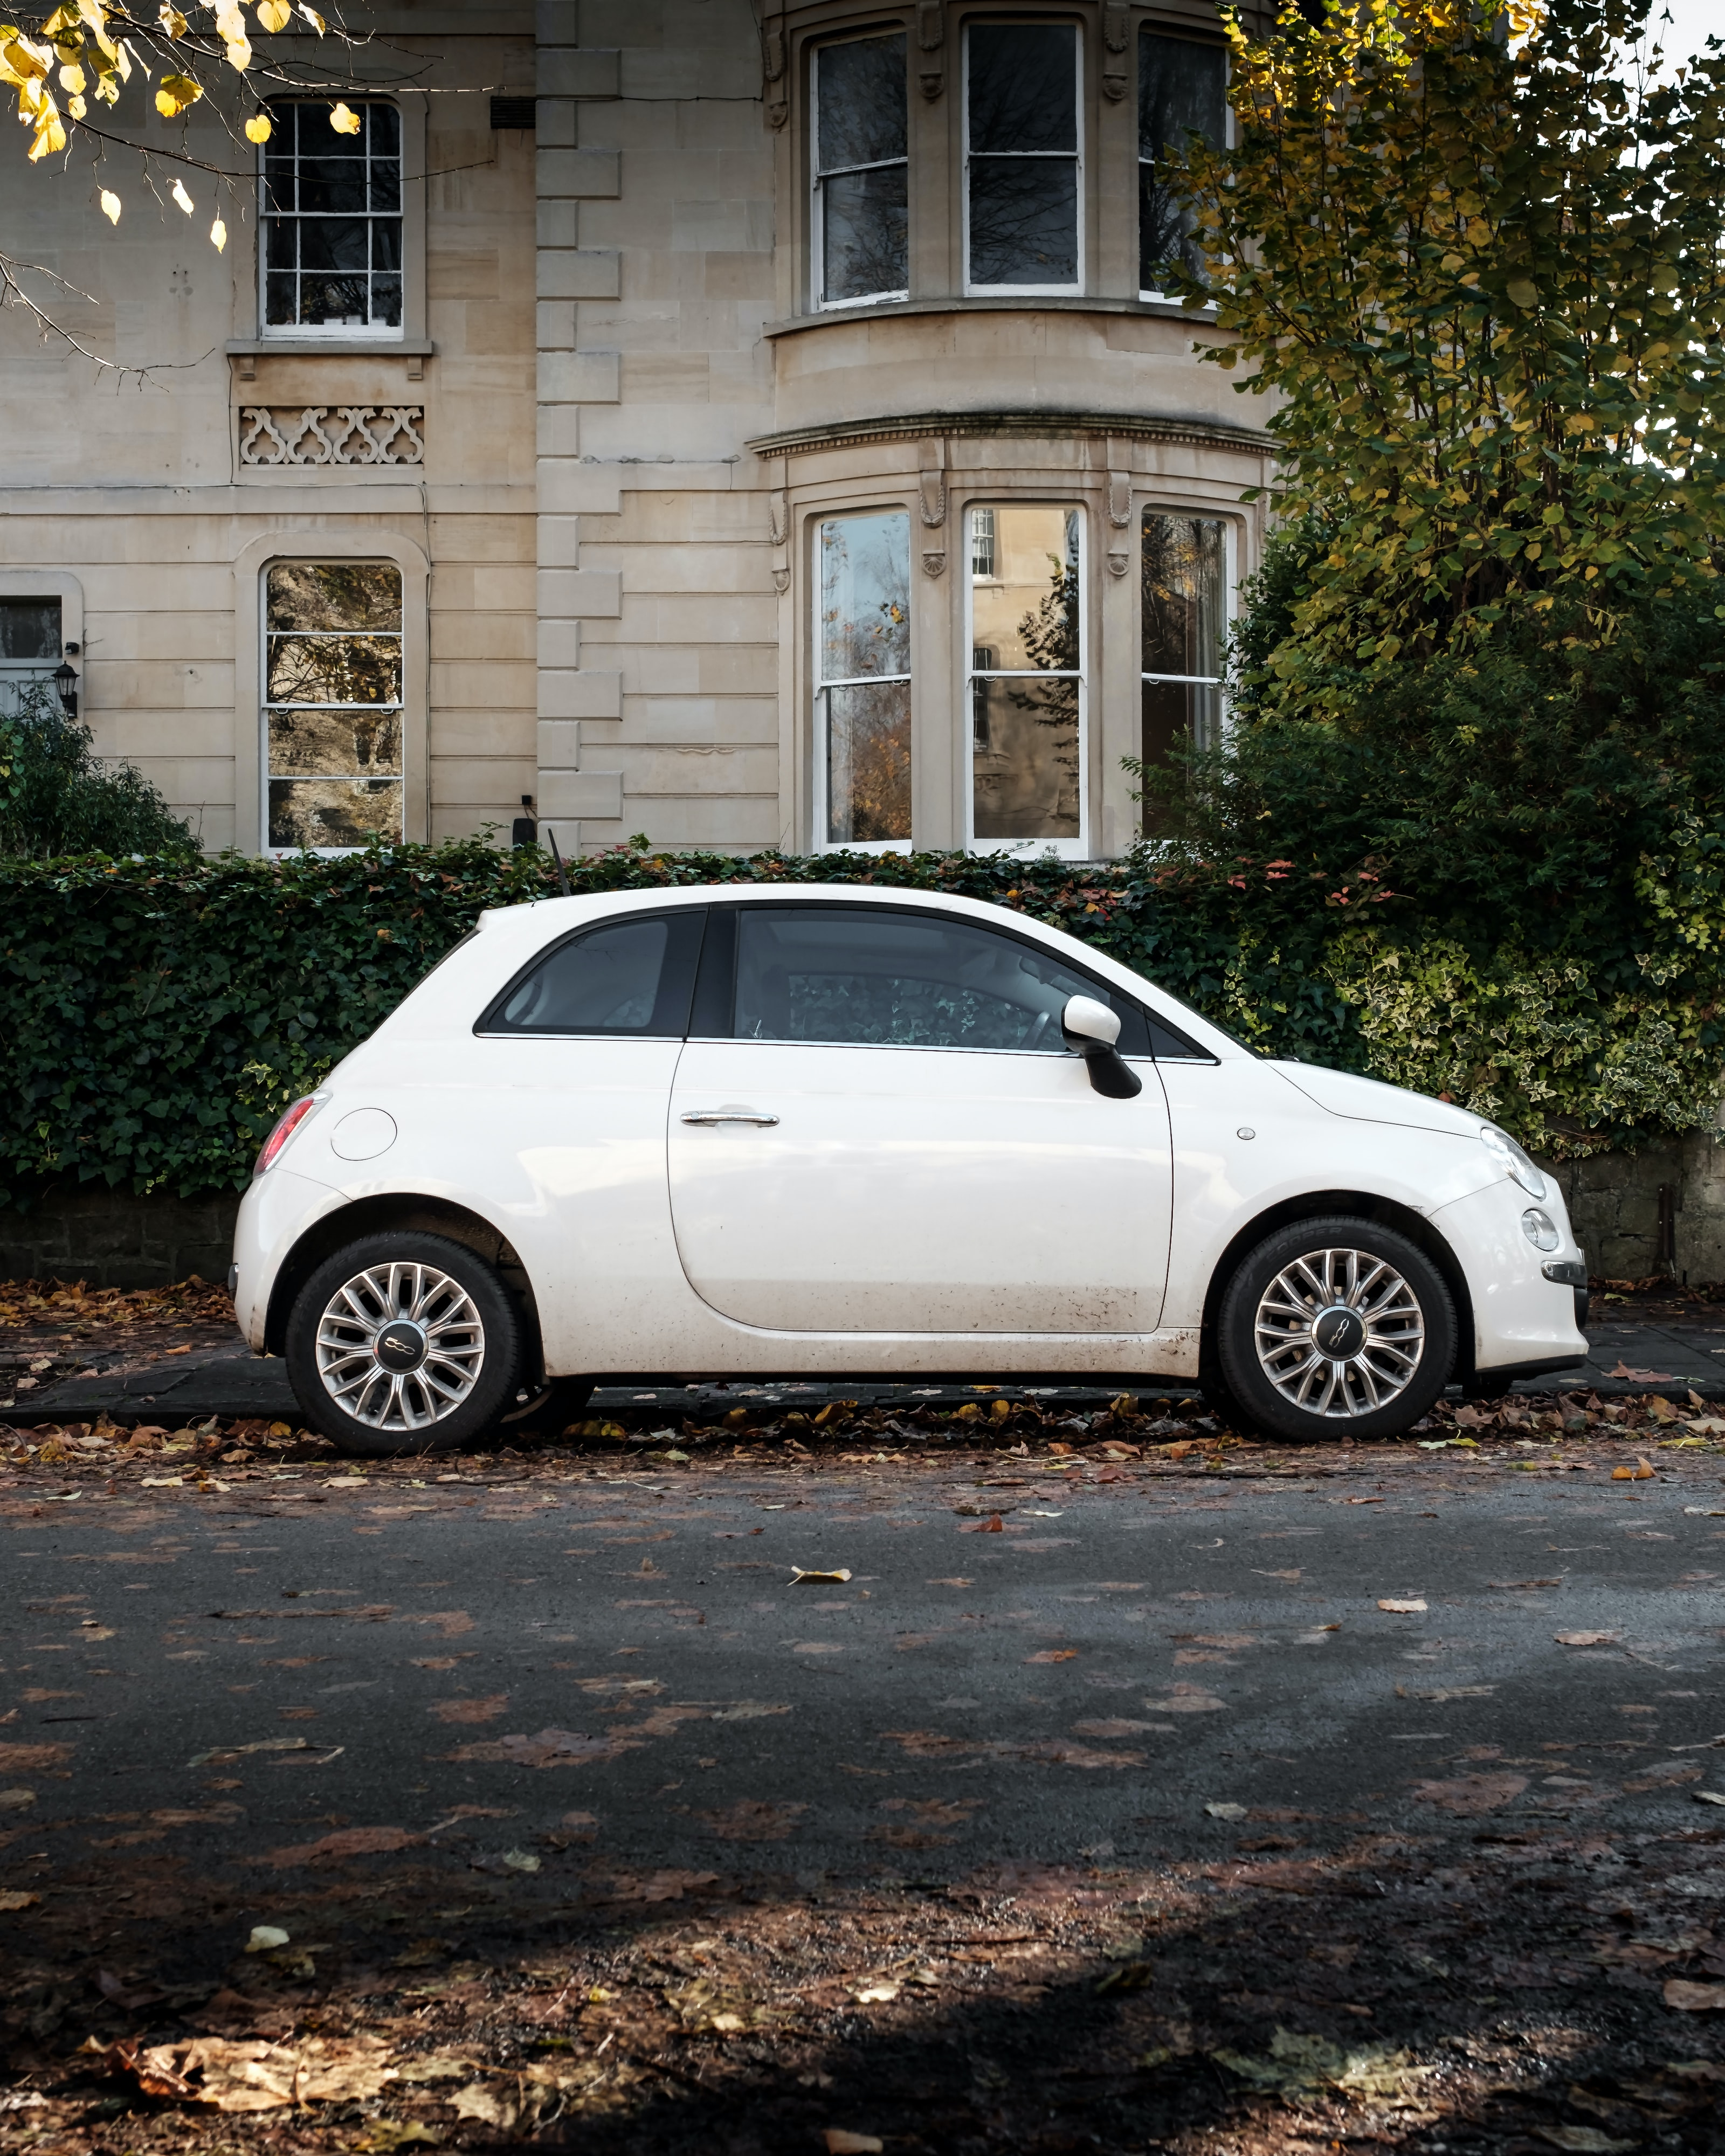
\includegraphics[width=0.7\columnwidth]{Image7}
\newline
\newline
\newline
\newline
\newline
\begin{tabular}{| m{3cm} | m{3cm} |}
\hline

Title  &  Value   \\

\hline
Camera Make  & FUJIFILM   \\
\hline
Camera Model  & X-T2   \\
\hline
Exposure time  & 1/80  \\
\hline
aperture & 5.6 \\
\hline


\end{tabular}


\end{center}

\pagebreak

\begin{center}
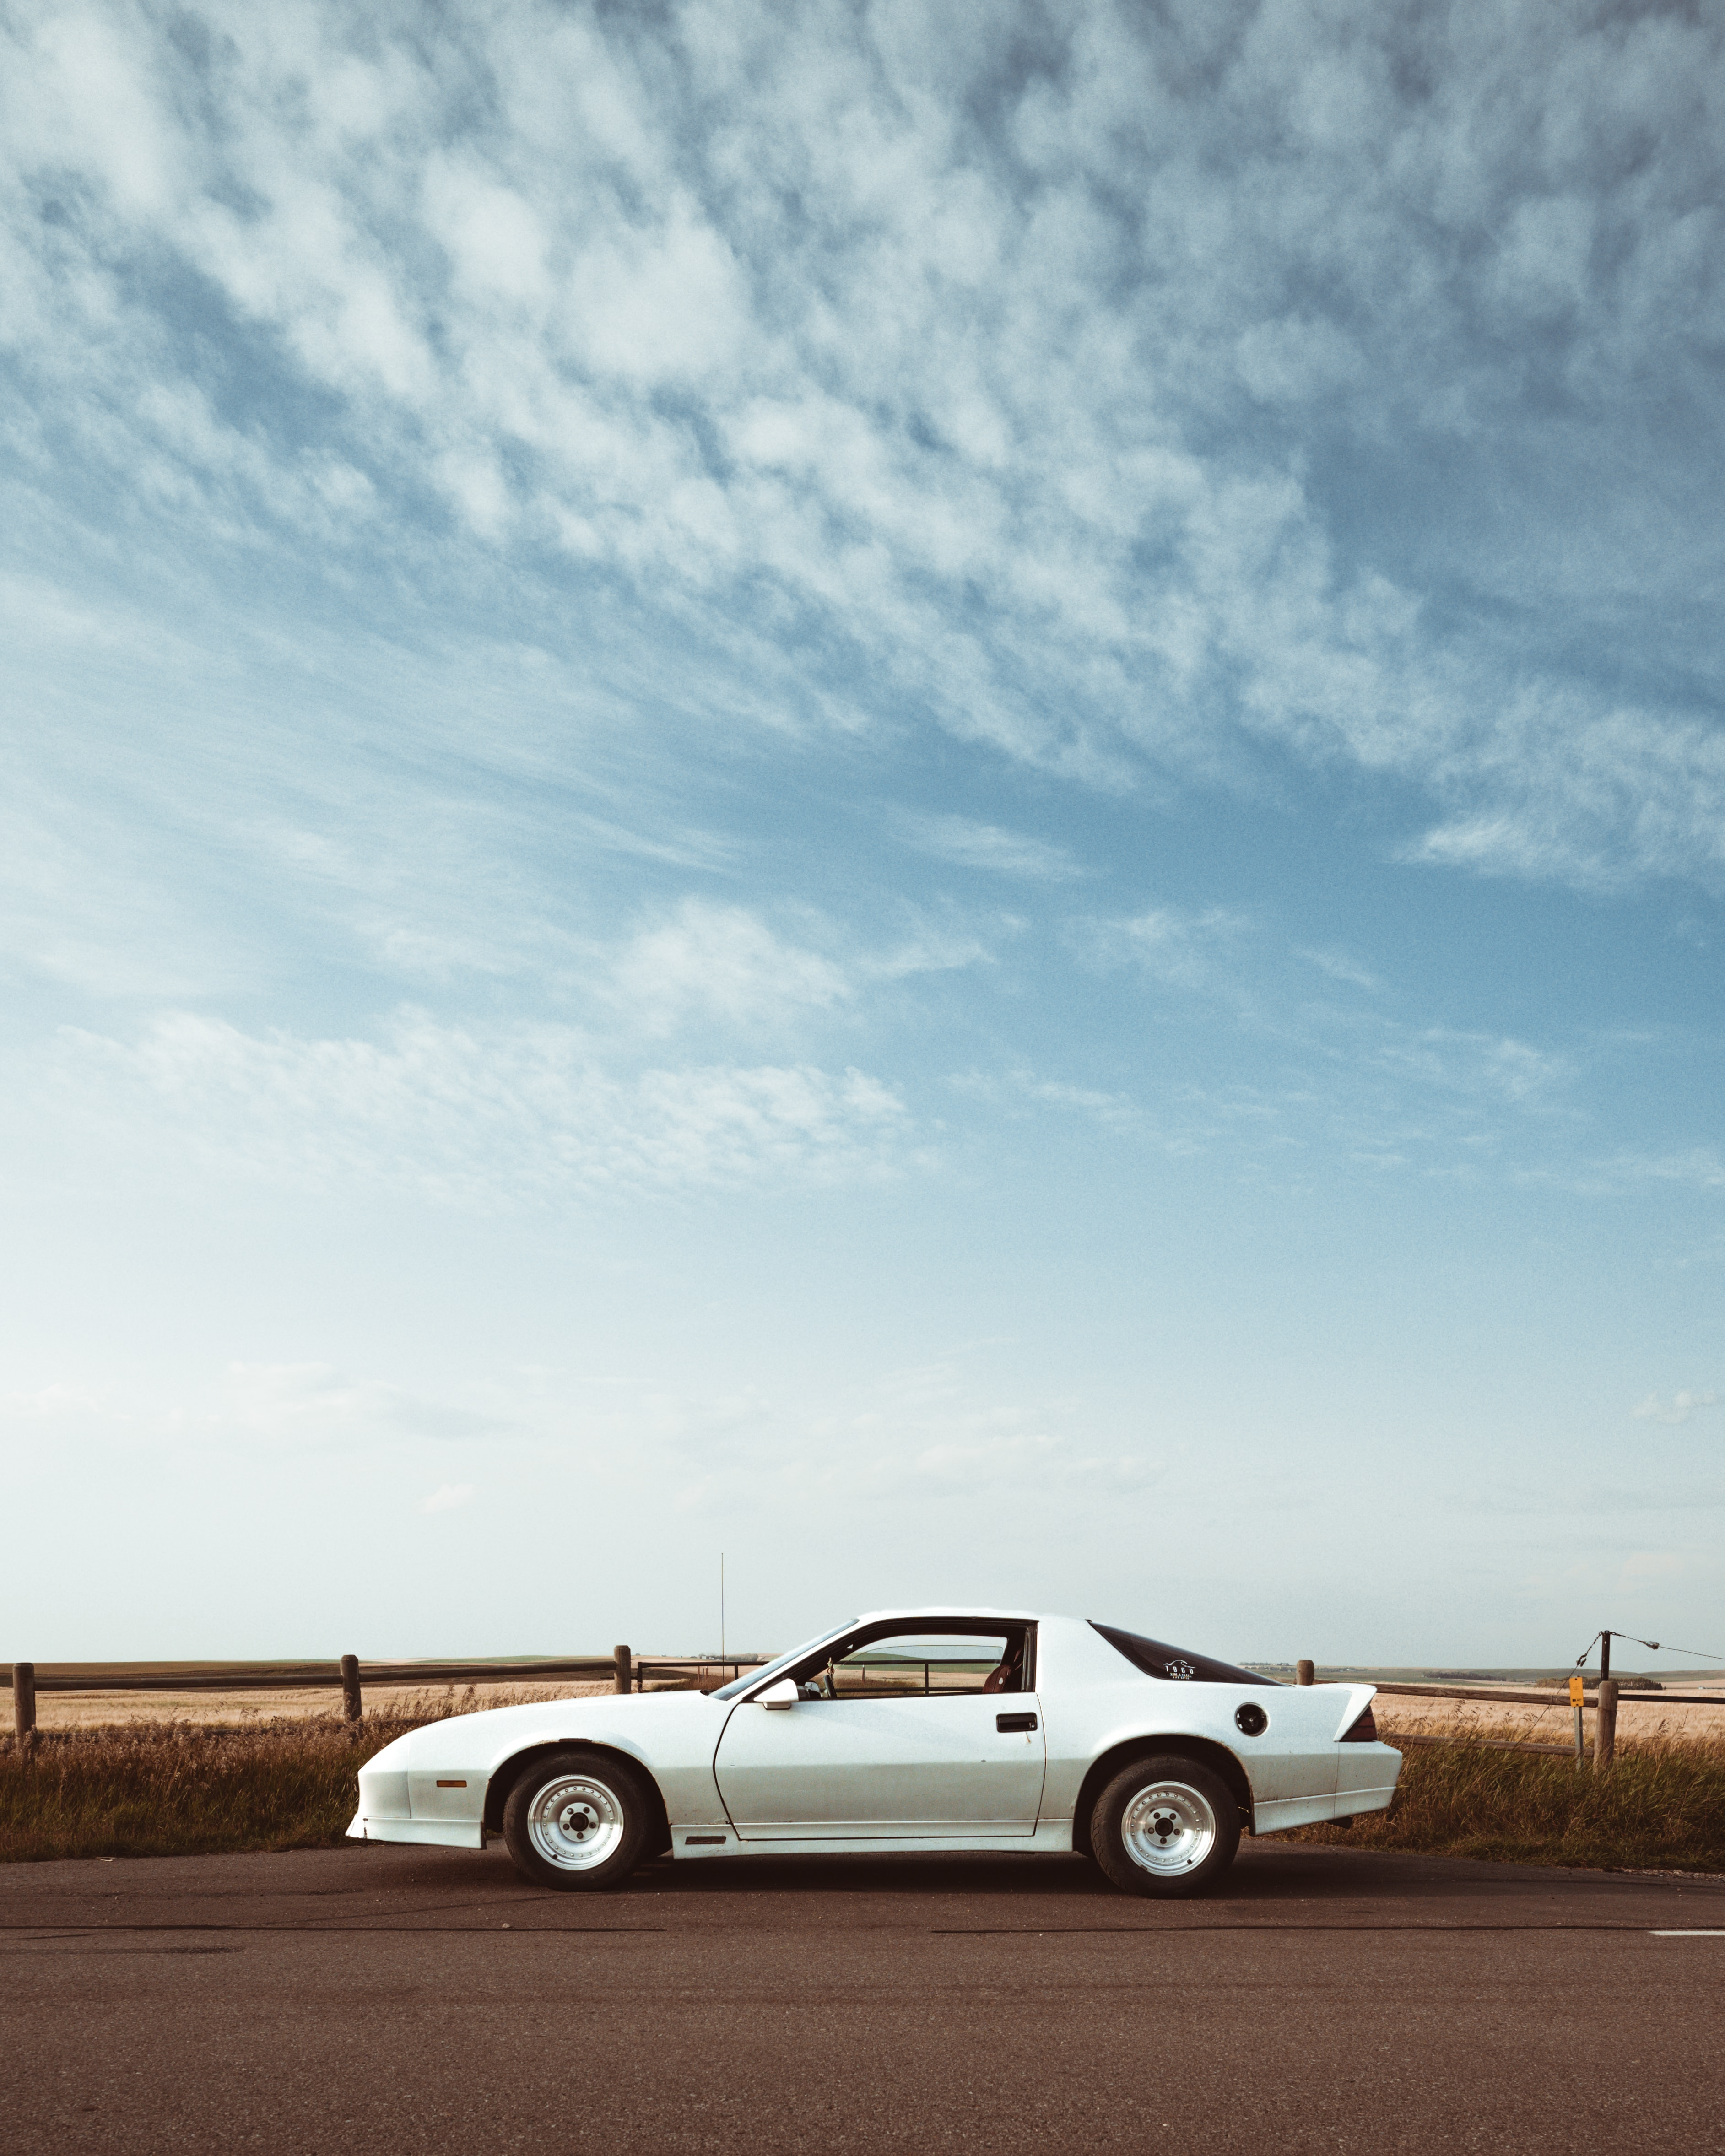
\includegraphics[width=0.7\columnwidth]{Image8}
\newline
\newline
\newline
\newline
\newline

\begin{tabular}{| m{3cm} | m{3cm} |}
\hline

Title  &  Value   \\

\hline
Camera Make  & SONY   \\
\hline
Camera Model  & ILCE-7RM2   \\
\hline
Exposure time  & 1/1250  \\
\hline
aperture & 5.0 \\
\hline

\end{tabular}


\end{center}

\newpage

\begin{center}
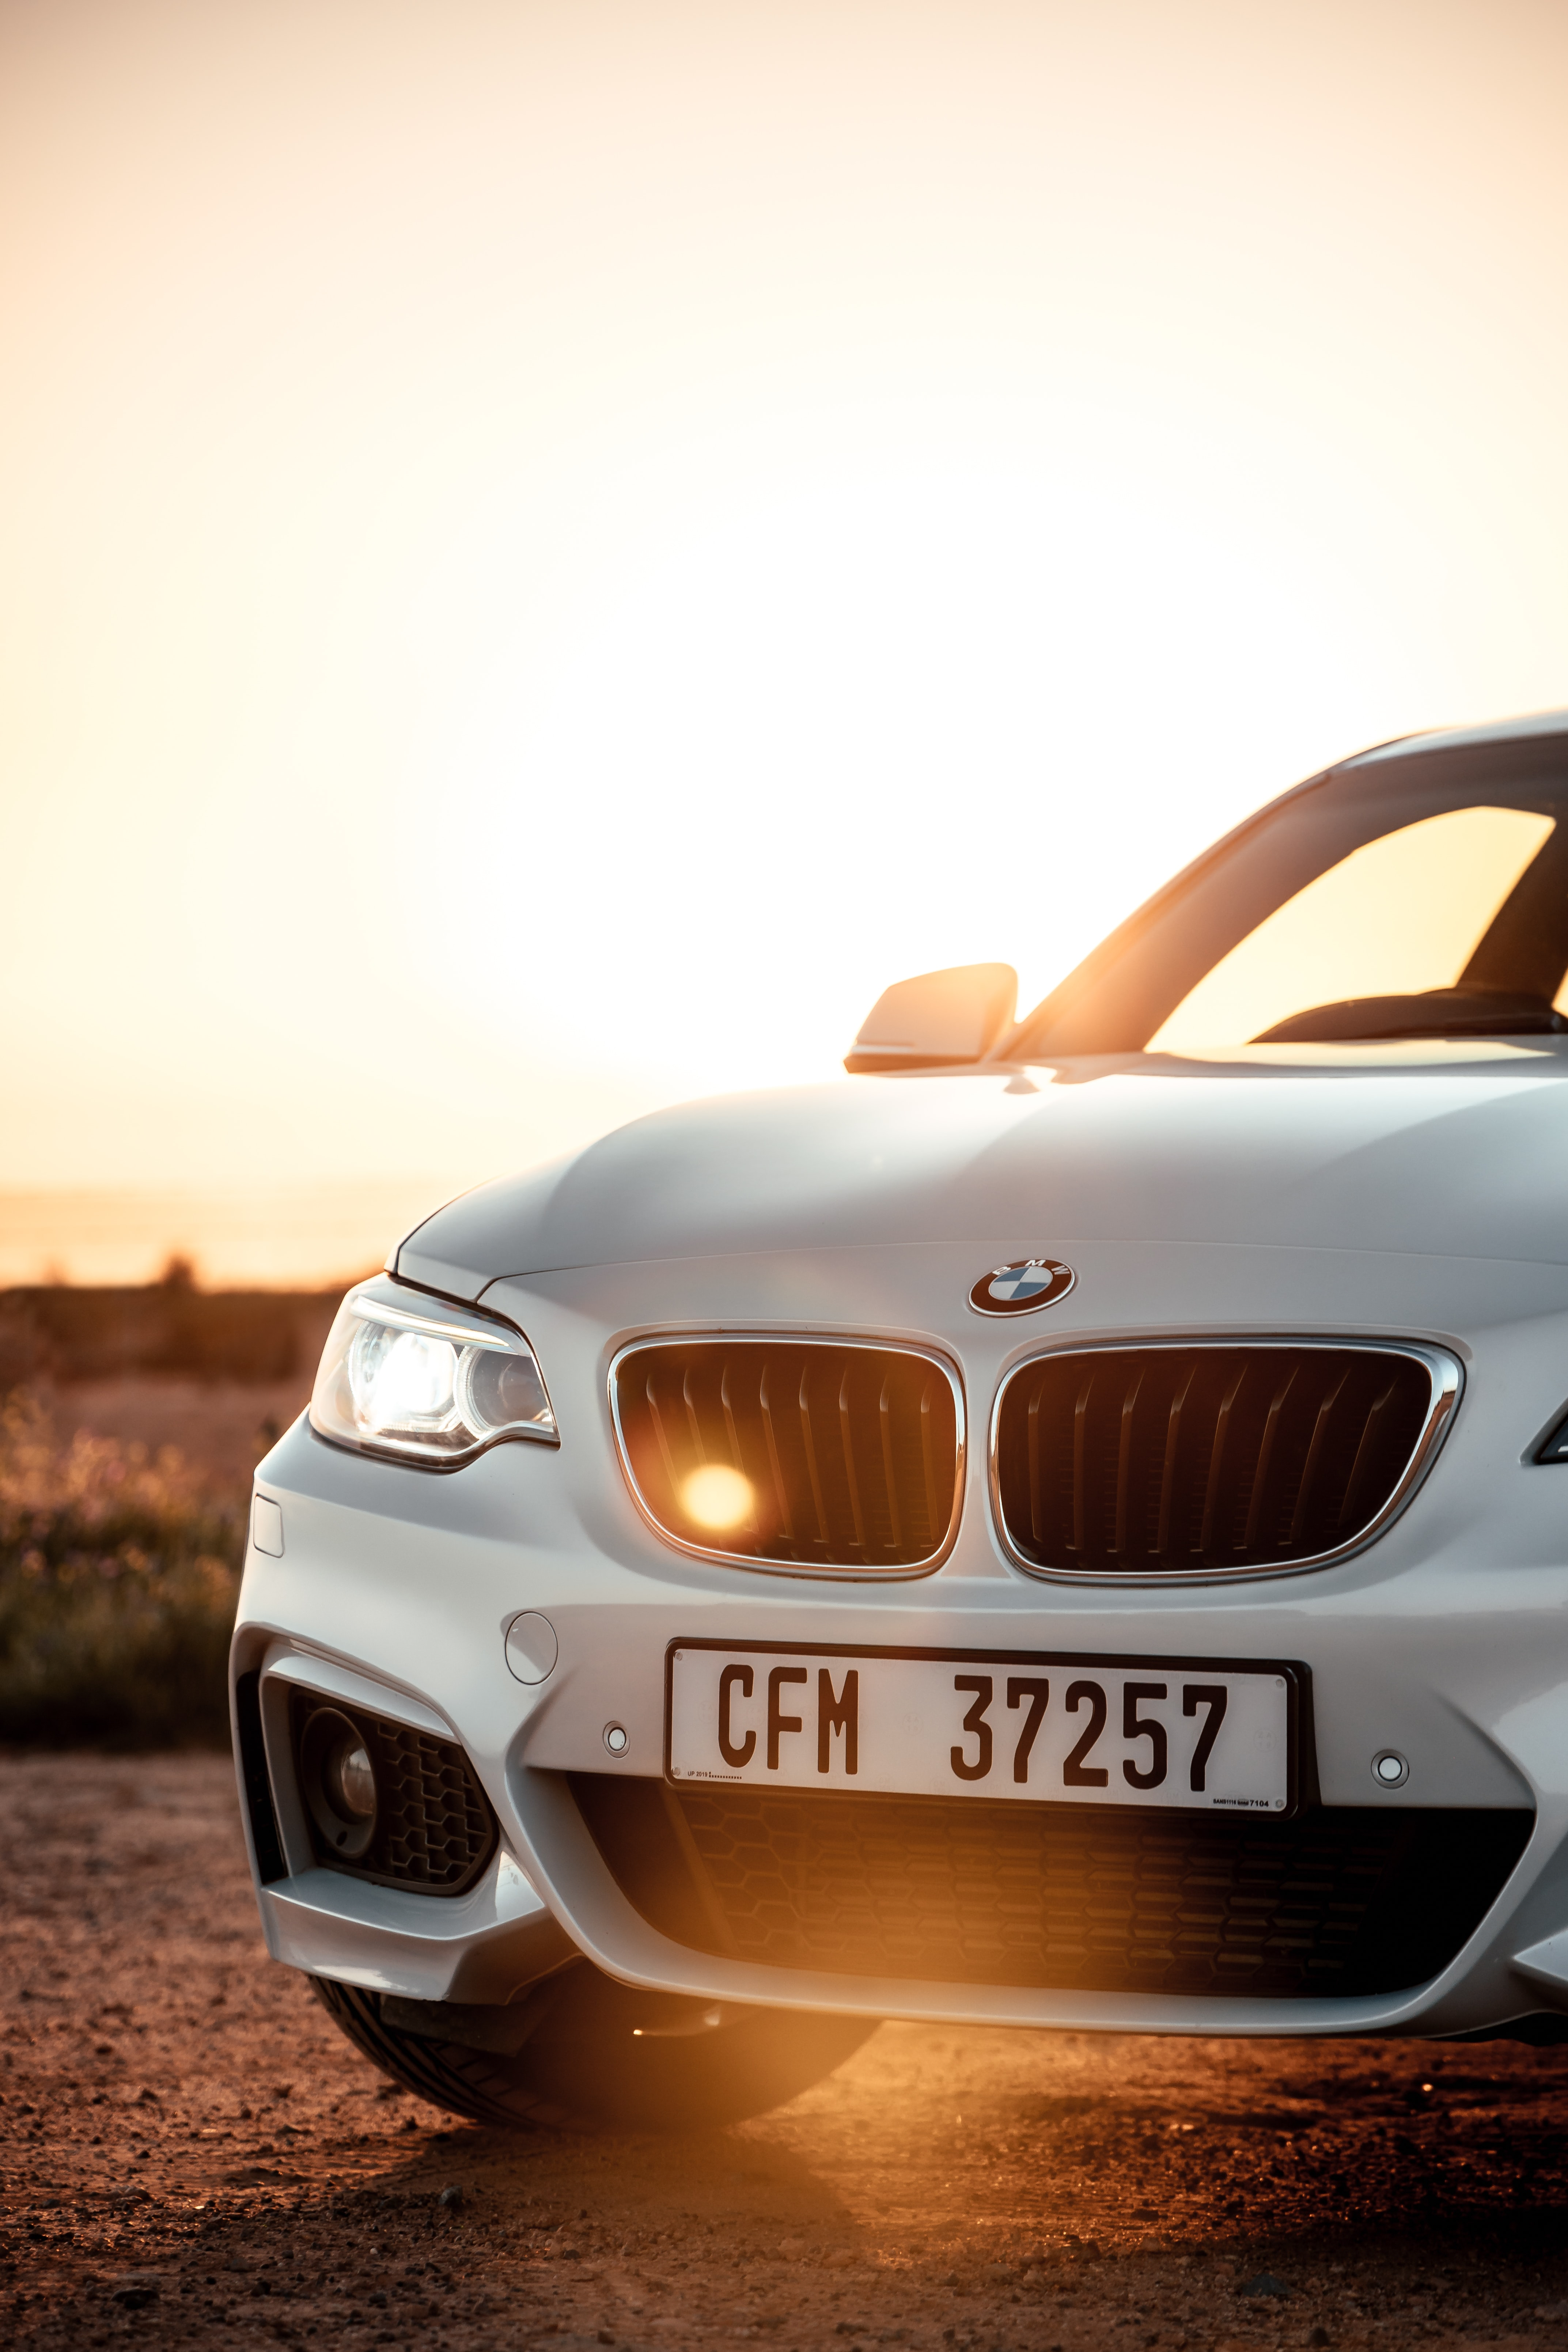
\includegraphics[width=0.7\columnwidth]{Image9}
\newline
\newline
\newline
\newline
\newline
\begin{tabular}{| m{3cm} | m{3cm} |}
\hline

Title  &  Value   \\

\hline
Camera Make  & Canon   \\
\hline
Camera Model  & Canon EOS R   \\
\hline
Exposure time  & 1/80  \\
\hline
aperture & 4.0 \\
\hline


\end{tabular}


\end{center}

\pagebreak

\begin{center}
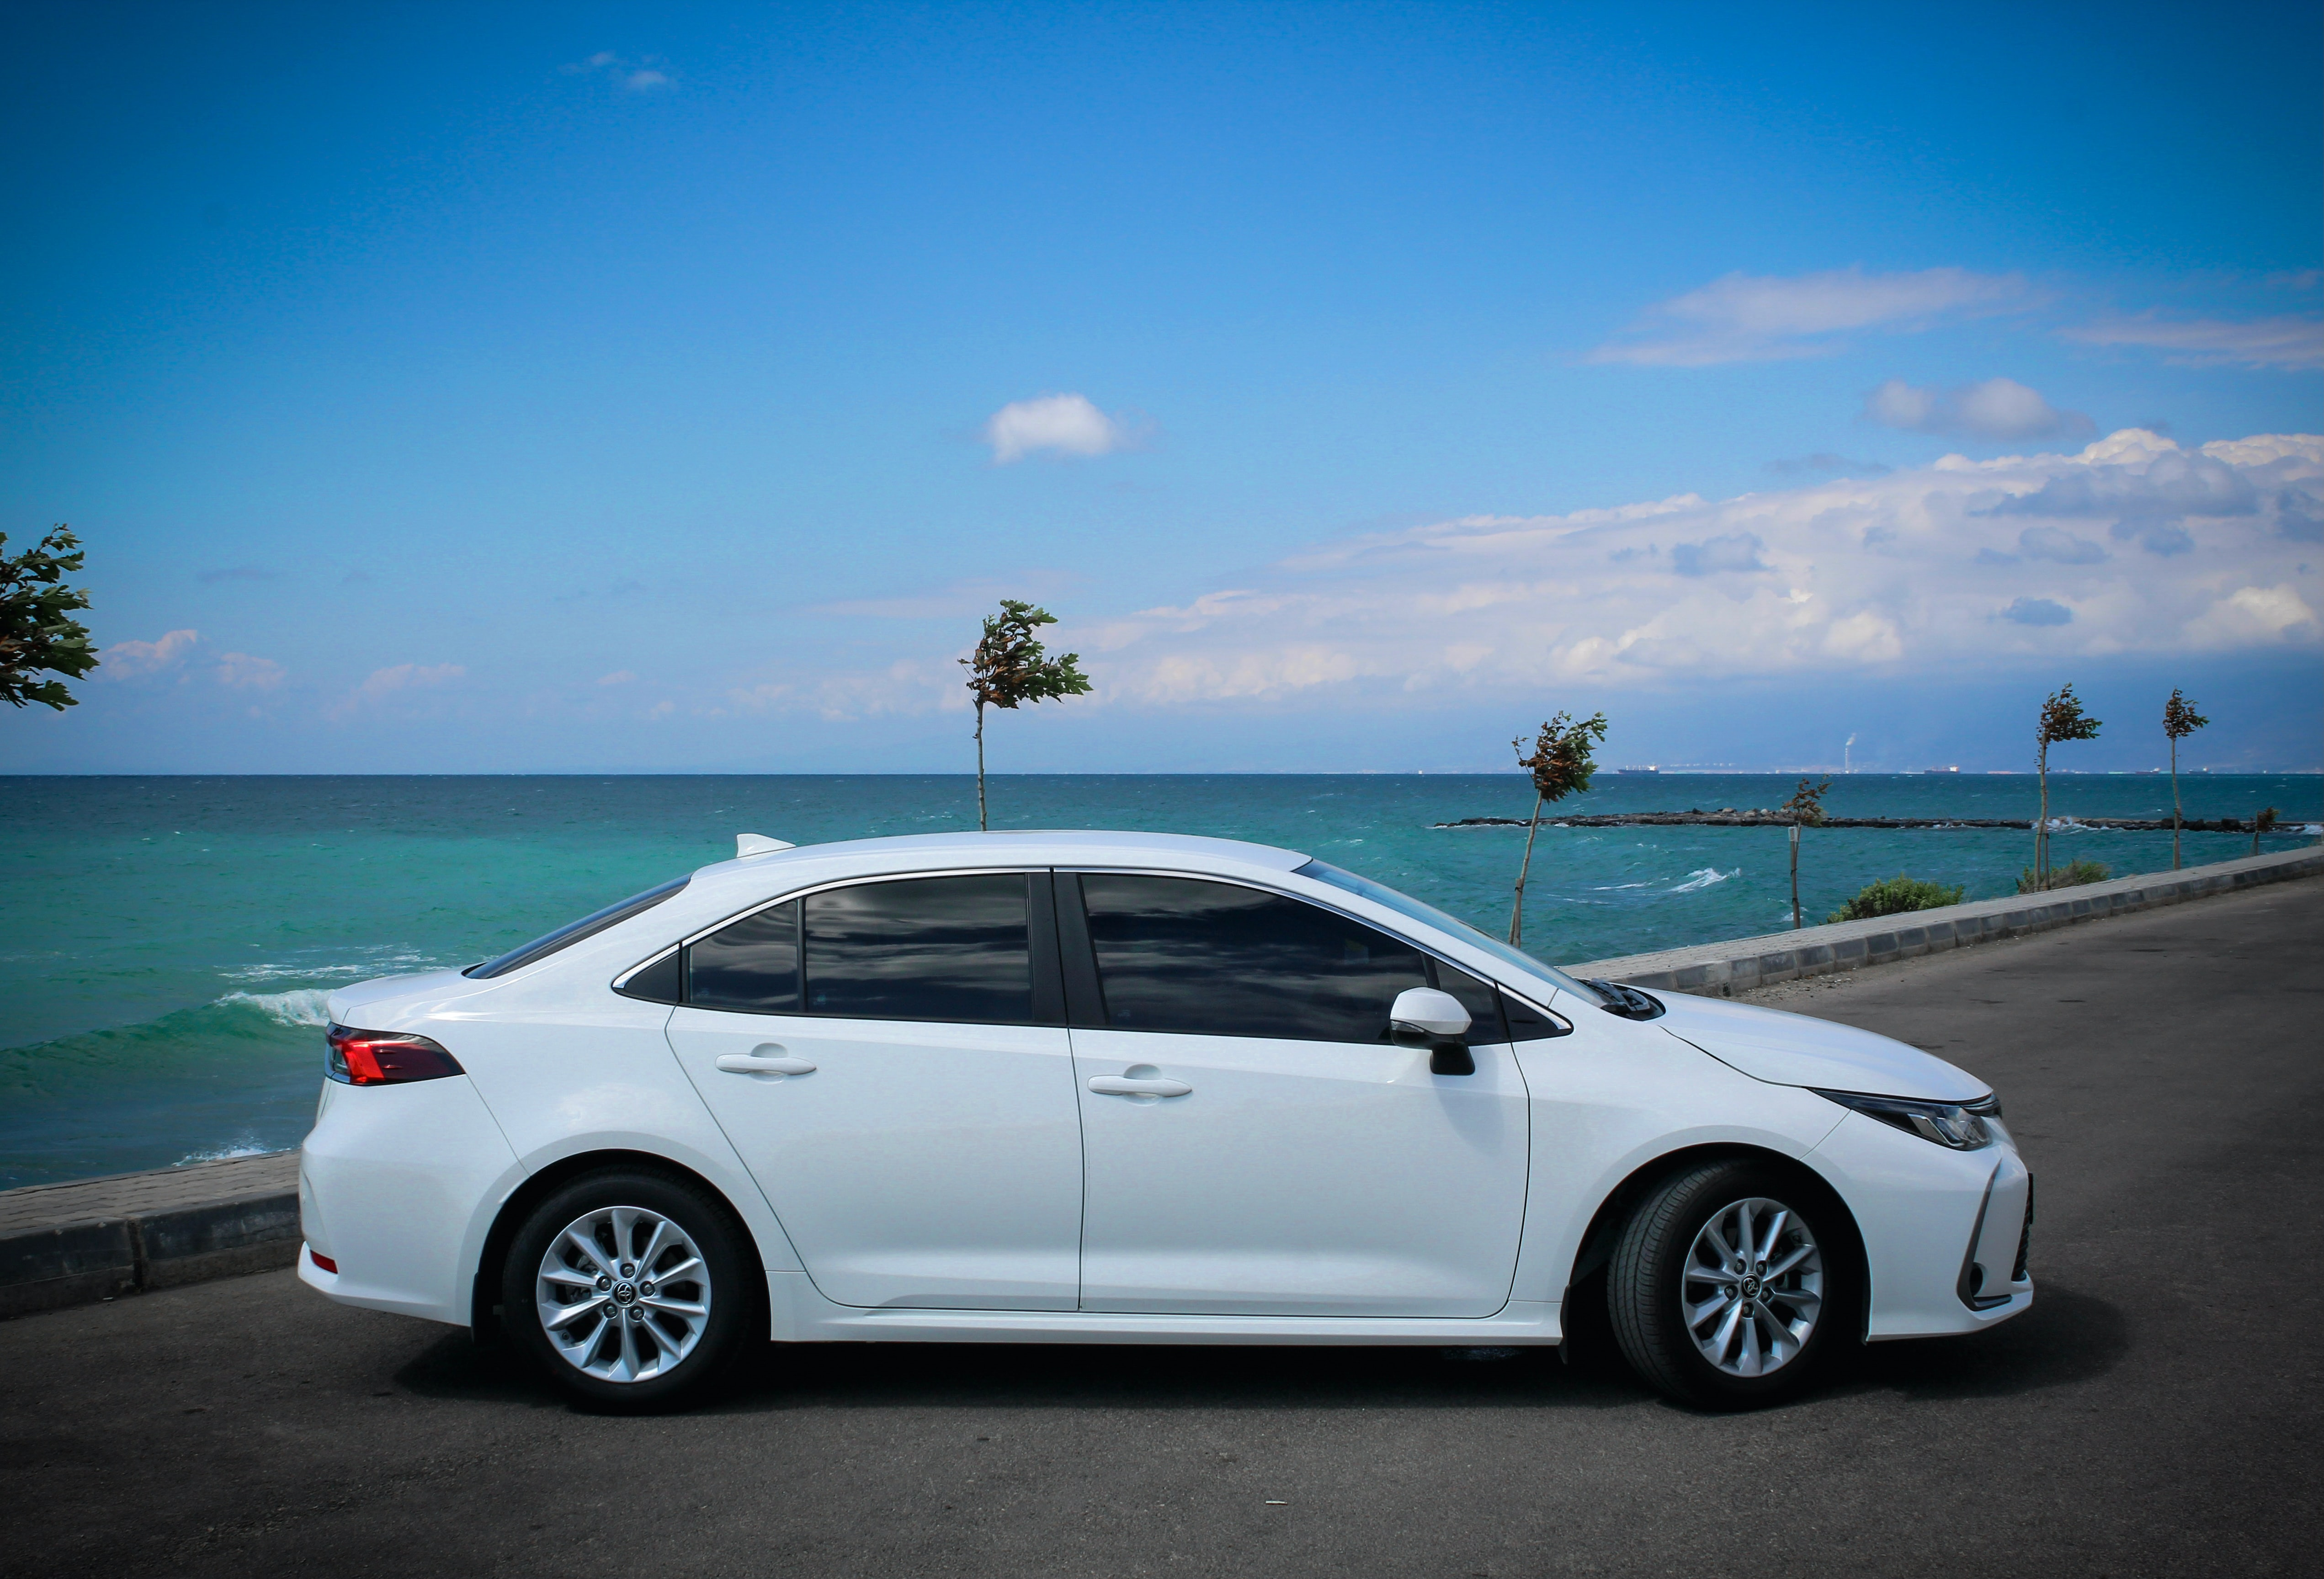
\includegraphics[width=0.7\columnwidth]{Image10}
\newline
\newline
\newline
\newline
\newline

\begin{tabular}{| m{3cm} | m{3cm} |}
\hline



Title  &  Value   \\

\hline
Camera Make  & Canon   \\
\hline
Camera Model  & Canon EOS 1200D   \\
\hline
Exposure time  & 1/200  \\
\hline
aperture & 7.6 \\
\hline

\end{tabular}


\end{center}


\end{document}